\documentclass[9pt,twocolumn,twoside,lineno]{pnas-new}
% Use the lineno option to display guide line numbers if required.

\templatetype{pnasresearcharticle} % Choose template 
% {pnasresearcharticle} = Template for a two-column research article
% {pnasmathematics} %= Template for a one-column mathematics article
% {pnasinvited} %= Template for a PNAS invited submission

\usepackage{amsmath}
\usepackage{tikz-dependency}
\DeclareMathOperator*{\argmax}{arg\,max}
\DeclareMathOperator*{\argmin}{arg\,min}
\DeclareMathOperator{\E}{\mathop{\mathbb{E}}}

\usepackage{amssymb}% http://ctan.org/pkg/amssymb
\usepackage{pifont}% http://ctan.org/pkg/pifont
\newcommand{\cmark}{\ding{51}}%
\newcommand{\xmark}{\ding{55}}%

%\usepackage{pslatex}
%\usepackage{latexsym}
\usepackage[english]{babel}
\usepackage[utf8]{inputenc}
\usepackage{bm}
\usepackage{graphicx}
\usepackage{tikz}
\usepackage{xcolor}
\usepackage{url}
%\usepackage[colorinlistoftodos]{todonotes}
\usepackage{rotating}
\usepackage{multirow}

\newcommand{\R}[0]{\mathbb{R}}
\newcommand{\Ff}[0]{\mathcal{F}}
\newcommand{\key}[1]{\textbf{#1}}


\newcommand{\soft}[1]{}
\newcommand{\nopreview}[1]{}
\newcommand\comment[1]{{\color{red}#1}}
\newcommand\mhahn[1]{{\color{red}(#1)}}
\newcommand{\rljf}[1]{{\color{blue}[rljf: #1]}}

\newcommand{\thetad}[0]{{\theta_d}}
\newcommand{\thetal}[0]{{\theta_{LM}}}
\newcommand{\thetap}[0]{{\theta_{P}}}


\title{Universals of word order result from optimization of grammars for efficient communication}

% Use letters for affiliations, numbers to show equal authorship (if applicable) and to indicate the corresponding author
%\author[a,1,2]{Michael Hahn}
%\author[a]{Daniel Jurafsky}
%\author[b]{Richard Futrell}

%\affil[a]{Stanford University}
%\affil[b]{University of California, Irvine}

% Please give the surname of the lead author for the running footer
\leadauthor{Hahn} 

% Please add here a significance statement to explain the relevance of your work
% limit 120 words 
\significancestatement{
What explains the universal properties of human languages? We present evidence that a major subset of these properties can be explained by viewing languages as codes for efficient communication among agents with highly generic cognitive constraints. In doing so, we provide the first full formalization and computational implementation of ideas which have been stated informally in the functional linguistics literature for decades. The success of this approach suggests a new way to conceptualize human language in quantitative and computational work, as an information-theoretic code dynamically shaped by communicative and cognitive pressures. Our results argue against the idea that the distinctive properties of human language result from essentially arbitrary genetic constraints.% (``universal grammar'').
}

% Please include corresponding author, author contribution and author declaration information
%\authorcontributions{MH and RF designed research. MH implemented models and experiments. MH and RF wrote the paper. MH, DJ, and RF provided comments on the paper.}
\authordeclaration{The authors declare no conflict of interest.}
%\equalauthors{\textsuperscript{1}A.O.(Author One) and A.T. (Author Two) contributed equally to this work (remove if not applicable).}
\correspondingauthor{\textsuperscript{2}To whom correspondence should be addressed. E-mail: mhahn2@stanford.edu}

% Keywords are not mandatory, but authors are strongly encouraged to provide them. If provided, please include two to five keywords, separated by the pipe symbol, e.g:
\keywords{language universals $|$ language processing $|$ computational linguistics} 

\begin{abstract}
%	TODO rewrite
The universal properties of human languages have been the subject of intense study across disciplines.
	We report novel computational and corpus-based evidence for the hypothesis that a prominent subset of these universal properties---those related to word order---result from a process of optimization for efficient communication among humans.
	We computationally formalize functional theories of language efficiencies using information theory and state-of-the-art machine learning techniques.
Applying these methods to data from 51 languages, we show that evolution towards efficiency results in word order patterns that predict a large subset of the major word order correlations reported in the linguistic typological literature.
%	TODO explain
	%We develop a probabilistic, differentiable model of word order grammars: the means by which different languages convert underlying hierarchical structures into strings of words.
	%We show how the parameters of a word order grammar can be optimized for efficiency of information transfer, quantified as a tradeoff between incremental predictability and mutual information with latent tree structures.
%	Applying these grammars to tree structures found in dependency corpora from 51 languages, we show that optimizing the grammar parameters for efficiency results in word order patterns that predict a large subset of the major word order correlations reported in the linguistic typological literature, and subsumes the predictions of previous heuristic theories such as dependency length minimization.
\end{abstract}

\dates{This manuscript was compiled on \today}
\doi{\url{www.pnas.org/cgi/doi/10.1073/pnas.XXXXXXXXXX}}


\begin{document}
% TODO mention the preregistration somewhere
\maketitle
\thispagestyle{firststyle}
\ifthenelse{\boolean{shortarticle}}{\ifthenelse{\boolean{singlecolumn}}{\abscontentformatted}{\abscontent}}{}


USE THE OTHER OVERLEAF VERSION
\crash{}


%Ray Jackendoff. 2002. Foundations of Language:
%Brain, Meaning, Grammar, Evolution. Oxford
%University Press, Oxford, UK


%William Croft and Alan Cruse. 2004. Cognitive
%Linguistics. Cambridge University Press, Cam-
%bridge, UK.
% --> emphasize language use

%Adele Goldberg. 2005. Constructions at work:
%The nature of generalization in language. Ox-
%ford University Press, Oxford, UK.
% --> emphasize usage-based grammar
% we are all born with the same basic conceptual apparatus, with the
%same basic communicative demands, and we all live in the physical world with
%forces of gravity, bodies, and night and day (cf. also LakoV 1987; Webelhuth and
%Ackerman 1998). Certain semantic/pragmatic functions are so relevant and
%useful that they can be found in language after language (Croft 2001).
%Cross-linguistic generalizations that relate form and function are explained
%by appeal to general cognitive constraints together with the functions of the
%constructions involved. Constructionists turn to grammar-external explan-
%ations such as universal functional pressures, iconic principles, and processing
%and learning constraints to explain such empirically observable cross-linguis-
%tic generalizations.
%For example, the fact
%that that most languages seem to have noun and verb categories may be
%explained by the existence of corresponding basic semantic categories (Baker
%2004). Hauser, Chomsky, and Fitch go so far as to suggest that the only innate
%ability speciWc to language that may be required are the recursive interfaces to
%phonology and semantics, and they allow that even these may turn out not to
%be speciWc to language (Hauser, Chomsky, and Fitch 2002).

% Haspelmath 1999 talks about types of explanations

%Joan Bresnan, Ash Asudeh, Ida Toivonen, and
%Stephen Wechsler. 2016. Lexical-Functional
%Syntax, 2nd ed. Blackwell, Malden, MA.


%Andrew Radford. 2006. Minimalist syntax re-
%visited. http://www.public.asu.edu/
%~gelderen/Radford2009.pdf.

%Givon

% TODO optimality theory and syntax citation?
%Blutner R. (2000) Some aspects of optimality in natural language interpretation. Journal of Semantics 17: 189–216

% ,lin2017critical
\dropcap{U}nderstanding and explaining the variation between human languages is the central  goal of Linguistics. % \cite{greenberg1963universals,chomsky1993lectures,givon2009genesis, ...}.
% behaghel1909beziehungen,
% \cite{behaghel1909beziehungen,zipf1949human,greenberg1963universals,lin2017critical} \cite{hawkins2007processing,bender2009linguistically,bender2013linguistic}
%An explanation for the universal properties of language would enable a deeper scientific understanding of what human language is and how to model it, with applications in psychology and natural language processing \cite{hawkins2007processing,bender2009linguistically,bender2013linguistic}.
% TODO mention universals here
Across theoretical paradigms, linguists have hypothesized that language is shaped by efficiency in computation~\cite{chomsky2005three,hauser2002faculty, berwick1984grammatical,hawkins1994performance} and communication~\cite{zipf1949human, Croft:Cruse:2004, Goldberg:2005, pinker1990natural, smith2013linguistic}.
%Role of general computational constraints ~\cite{hauser2002faculty} % berwick2016only
In this work we examine this question from a computational perspective, demonstrating a fully formalized and implemented framework in which a large class of language universals can be explained through the computational optimization of grammars for efficiency. % information-theoretic 
Specifically, we show that efficiency optimization explains  linguistic universals related to word order first documented by Greenberg \cite{greenberg1963universals}. 
% TODO change wording so it's clear that this is a very major thing


% Things TODO
% - make clear that efficiency is something both functional and generative linguists have been appealing to
% - at some point address head direction idea
%TODO at some point address head direction idea
%    - Vennemann 1972, 1974ab, 1976
%    -Hawkins 1980 limitations of head direction, also Hawkins 1982


%foreshadow functional explanations?
%
%- these linguistic patterns reflect general principles of communication
%
%- big idea has been around for a long time
%
%- here for the first time direct computational test
%
%- we can predict broad patterns, and make language-specific predictions based on these general principles 
%

% TODO add a cogsci person to citation chain at the beginning


%\dropcap{F}or decades, researchers in fields ranging from philology to cognitive science to statistical physics have been involved in documenting and trying to explain the universal syntactic and statistical properties of human language \cite{behaghel1909beziehungen,zipf1949human,greenberg1963universals,lin2017critical}. An explanation for the universal properties of language would enable a deeper scientific understanding of what human language is and how to model it, with applications in psychology and natural language processing \cite{hawkins2007processing,bender2009linguistically,bender2013linguistic}.



%Berwick and Chomsky ‘gene rative process  is optimal  ’, ‘efficient computa  tion ’(71), ‘this newly  emerged  computationalsystem forthought  ...ispe rfe ct, in sofar asSMT is corr ect ’(80).  ‘op -tim al’or ‘effici ent ’or ‘per fect ’. 

%Chomsky Three Factors, 2003:
% --> emphasizes 'computational efficiency'

%\textbf{TODO maybe should be more general in the beginning, as in the first version. Also make sure the reader doesn't think 'it's just headedness, why bother'.}

%We aim to explain the linguistic universals related to word order first documented by Greenberg \cite{greenberg1963universals}. 
Human languages vary in the order in which they express information.
Consider Figure~\ref{fig:arabic-japanese-simple}, showing a sentence in Arabic (top) and Japanese (bottom), both translating to `I wrote a letter to a friend.'
Both sentences contain a verb meaning `wrote', a noun expressing  the object `letter', and an adpositional phrase translating to `to a friend'.
%In linguistic terminology, `letter' is the object of the verb, whereas the phrases translating as `to a friend' are known as adpositional phrases.
Yet, the order of these words are entirely different in the two languages:
%However, the languages differ in the order in which these words and phrases are arranged: 
The verb stands at the beginning in Arabic, and at the end in Japanese.
Arabic expresses `to' by a \emph{preposition} (\emph{preceding} the noun `friend'); Japanese uses a \emph{postposition} (\emph{following} it). % and a postposition in Japanese, following `friend'.

This variation reflects a deep and stable regularity:
While languages ordering the objects before (Japanese) or after (Arabic) the verb are approximately equally common around the world,
this is strongly correlated with the occurrence of pre- or postpositions (Figure~\ref{fig:corr-table}, top):
Languages ordering their objects the way Japanese does, have postpositions; languages ordering them as Arabic does have prepositions.



\begin{figure}
    \centering
    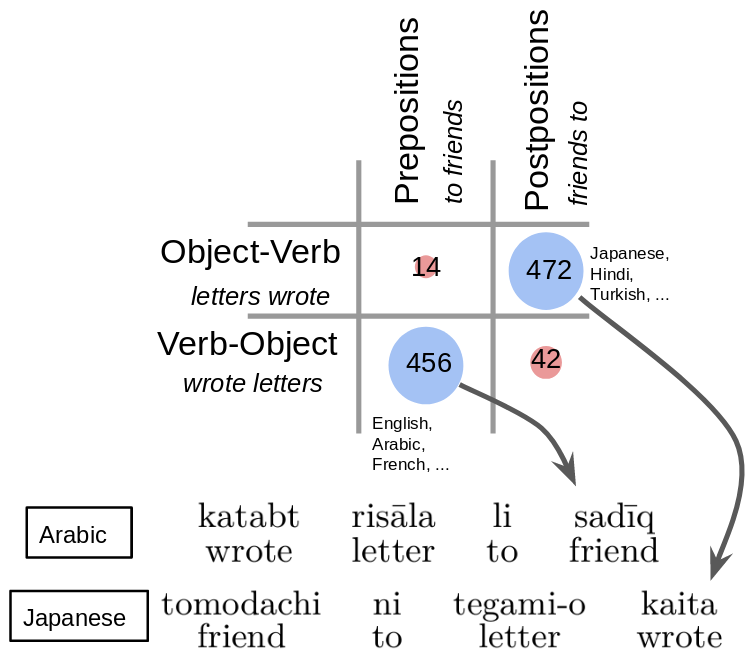
\includegraphics[width=0.4\textwidth]{figures/corr-full.png}
\caption{ The concept of a word order correlation: Languages can order the object after (Arabic) or before (Japanese) the verb, and have prepositions (Arabic) or postpositions (Japanese). For each combination, we indicate how many languages satisfy it, as documented in the World Atlas of Language Structure~\cite{wals}. Combinations on the diagonal are vastly more common than off-diagonal ones. % A sentence in Arabic (top) and Japanese (bottom), translating to `I wrote a letter to a friend.' Note the reversal of word order: Arabic has verb-object order and prepositions, while Japanese has object-verb order and postpositions.
	}\label{fig:arabic-japanese-simple}	\label{fig:corr-table}
\end{figure}



This generalization falls in a group of language universals that were originally documented by Greenberg \cite{greenberg1963universals}, known as \key{word order correlations}:
These describe correlations between the relative positions of different types of expressions across languages.
The example above documents that the position of the object (`letter') relative to the verb is \key{correlated} with the position of the adposition (`to'). %adpositional phrases (`to a friend') relative to the verb.
Greenberg also found that the order between verb and object is correlated with other aspects of a language's word order (Table~\ref{table:corr-dryer}), such the order of verb and adpositional phrase (`wrote -- to friend' in Arabic vs `friend to -- wrote' in Japanese), and that of noun and genitive (`book -- of friend' in Arabic, `friend of -- book' in Japanese).




Supported by languages on all continents, these correlations are among the language universals with the strongest empirical support.
Importantly, their validity is also independent from specific assumptions about theories of grammar.



Explaining these patterns has been an important aim of linguistic research since Greenberg's seminal study~\cite{lehmann1973structural, vennemann1974theoretical,jackendoff1977x,frazier1985syntactic,chomsky1988language, dryer1992greenbergian, hawkins1994performance}.



A prominent line of research has argued that language universals arise for \key{functional} reasons: that is, because they make human communication and language processing maximally efficient, and regularities across languages hold because these efficiency constraints are rooted in general principles of communication and cognition (e.g., \cite{gabelentz1901sprachwissenschaft,zipf1949human,hockett1960origin,givon1991markedness,hawkins1994performance,hawkins2004efficiency,hawkins2014crosslinguistic,croft2001functional,haspelmath2008parametric,jaeger2011language}).
Under this view, the various human languages represent multiple solutions to the problem of efficient information transfer given human cognitive constraints.

Zipf \cite{zipf1949human} argued that language optimizes a tradeoff between the Forces of \emph{Unification} and \emph{Diversification}.
The Force of Unification is a pressure to reduce the complexity of the language to make production and processing as easy as possible.
Conversely, the Force of Diversification favors languages that provide different utterances for different meanings, so that the listener can unambiguously identify the meaning from the utterance.
These two forces act in opposing directions:
Producing and processing simple utterances incurs little cost, but more complex and diverse utterances are required in order to provide higher informativity.
The idea that many properties of language arise from the tension between these two pressures has a long and fruitful history in theoretical studies of language~\cite{gabelentz1901sprachwissenschaft,horn1984toward, lindblom1990explaining, schwartz1997dispersion, hawkins2004efficiency}.


Recent work has used an information-theoretic formalization to computationally test these ideas in various domains of language, showing that they predict
both basic statistical properties of languages~\cite{ferreri2003least} and language development~\cite{smith2013linguistic},
and sophisticated aspects of language, such as pragmatic inference \cite{frank2012predicting}, and the distribution of color words~\cite{zaslavsky2018efficient} and kinship categories~\cite{kemp2012kinship} across many languages.


While it has been suggested that these ideas should also apply to grammar~\cite{hawkins2004efficiency}, testing these accounts is more difficult in the domain of grammar, as this requires both large amounts of data representative of language use across languages and cultures, and computational methods for estimating the efficiency of entire languages.
In this work, we address these challenges by combining large-scale text data from 51 languages with state-of-the-art machine learning techiques to estimate the communicative efficiency of grammar.
We apply this approach to the problem of explaining Greenberg's word order correlation universals.
We first show that the word order of languages has evolved to optimize efficiency.
We then show that efficiency optimization accounts for the Greenbergian word order correlations, and makes fine-grained per-language predictions about individual syntactic patterns.
Our results show how general properties of efficient communication gives rise to the universal word order properties of human language.




\begin{table}
	\begin{center}
%		\setlength\tabcolsep{1.5pt}
\begin{tabular}{|c|ll|ll|}
	\hline
	%&
	&	\multicolumn{2}{c|}{\textbf{Arabic} (English, ...)}   &        \multicolumn{2}{c|}{\textbf{Japanese} (Hindi, ...)} \\ \hline\hline
	& \multicolumn{2}{c}{Correlates with...} & \multicolumn{2}{|c|}{Correlates with...}  \\
	&	Verb & Object     & Object & Verb    \\ \hline\hline
	& kataba & rasaa'il 	&tegami-o & kaita \\
	&	\emph{wrote} & \emph{letters} & 	\emph{letter} & \emph{wrote} \\ \hline 
	\multirow{2}{*}{\raisebox{.5pt}{\textcircled{\raisebox{-.9pt} {1}}}}	&	li    &    sadiiq       &	tomodachi & ni \\
	&		\emph{to}            & \emph{a friend} &		\emph{friend} & \emph{to} \\ \hline
	\multirow{2}{*}{\raisebox{.5pt}{\textcircled{\raisebox{-.9pt} {2}}}}	&kaana    &    sadiiq         &	tomodachi & datta \\
	&	\emph{was}        & \emph{a friend} 	&\emph{friend} & \emph{was} \\ \hline
	\multirow{2}{*}{\raisebox{.5pt}{\textcircled{\raisebox{-.9pt} {3}}}}	&sawfa    &    yaktub       & 	kak & udesho \\
	&	\emph{will}          & \emph{write}  &    	\emph{write} & \emph{will} \\ \hline
	\multirow{2}{*}{\raisebox{.5pt}{\textcircled{\raisebox{-.9pt} {4}}}}	& sadiiq  &    John    & 	John no & tomodachi \\
	&	\emph{friend} &  \emph{of John}  &	\emph{John of} & \emph{friend} \\ \hline
	\multirow{2}{*}{\raisebox{.5pt}{\textcircled{\raisebox{-.9pt} {5}}}}	&kutub    &    taqra'uha       & 	anata-ga yonda & hon \\
	&	\emph{books} & \emph{that you read}  &	\emph{that you read} & \emph{book} \\ \hline
	\multirow{2}{*}{\raisebox{.5pt}{\textcircled{\raisebox{-.9pt} {6}}}}	&'an    &    tusil        & 	toochaku suru & koto \\
	&	\emph{that} & \emph{she arrives}  &	\emph{has.arrived} & \emph{that} \\ \hline
	\multirow{2}{*}{	\raisebox{.5pt}{\textcircled{\raisebox{-.9pt} {7}}}}	&dhahabt	    &    'ila lmadrasa     & 	gakkoo ni & ittekimashita \\
	&	\emph{went} & \emph{to school}  &	\emph{school to} & \emph{went} \\ \hline
	\multirow{2}{*}{\raisebox{.5pt}{\textcircled{\raisebox{-.9pt} {8}}}}	&'uriid    &    'an 'ughaadir         & 	yom & itai \\
	& \emph{wants}   &  \emph{to leave}  &	\emph{to leave} & \emph{want} \\ \hline \hline
\end{tabular}
	\end{center}
	\caption{Greenberg's word order correlations, exemplified by Arabic (left) and Japanese (right) examples: Across the world, the orders of different constituents are strikingly correlated with that of verb and object. See Materials and Methods.}\label{table:corr-dryer}
\end{table}





\section{Formalizing Efficiency in Word Order}


\begin{figure}
    \centering
    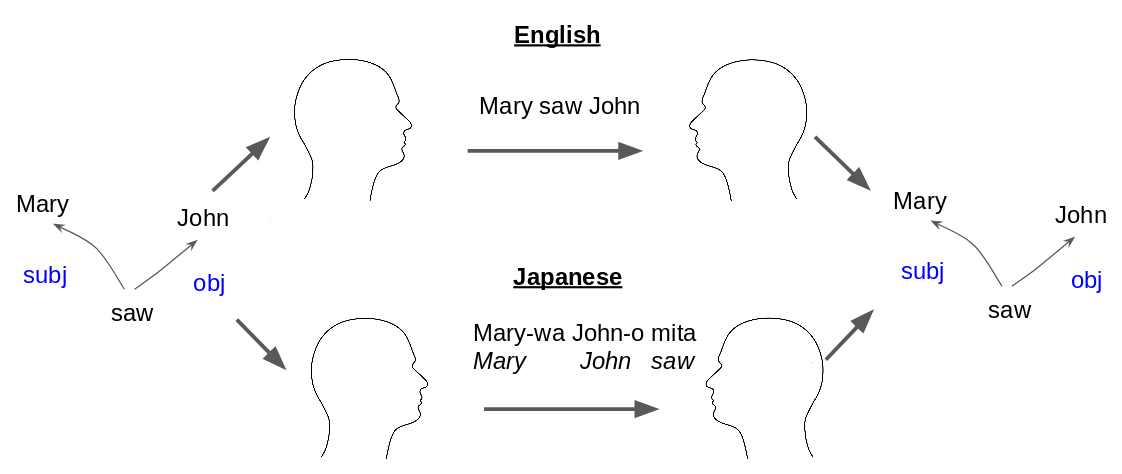
\includegraphics[width=0.45\textwidth]{figures/communication-two-langs.png}
	\caption{Grammars define communication channels: A speaker (left) expresses a dependency structure into a string of words forming a sentence. The order of words is determined by the grammar of the language. A listener recovers a dependency structure. Communication is successful if the listener recovers the correct depenency structure.}
	\label{fig:comm}
\end{figure}



% Given a set of dependency structures, grammars define a set of sentences. Each grammar defines a consistent ordering for the different kinds of syntactic relations, e.g., 
\begin{figure}
    \centering
    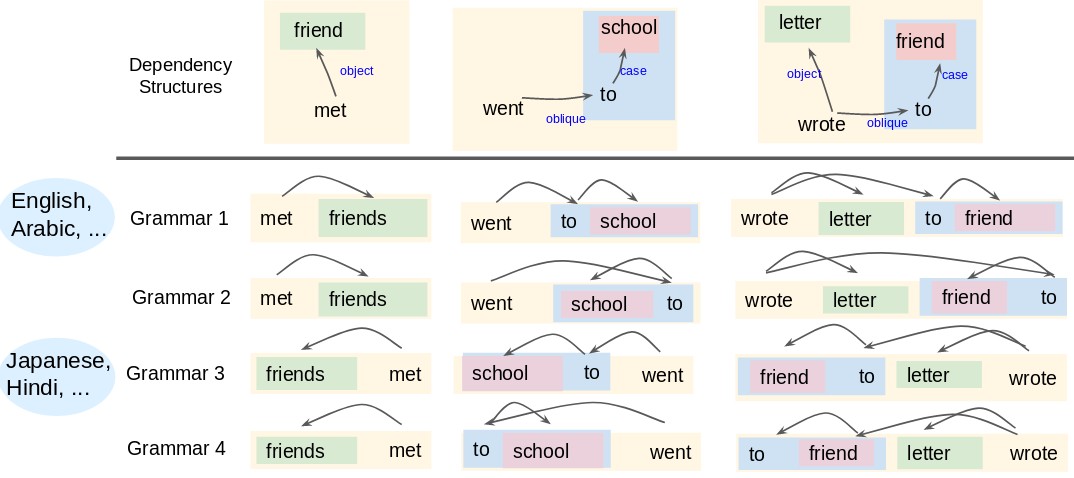
\includegraphics[width=0.45\textwidth]{figures/grammars-langs.png}
	\caption{Grammars define consistent ordering rules for dependency structures. Here, Grammars 1 and 2 order the object after the verb, Grammars 3 and 4 order the object before the verb. Grammars 1 and 3 conform to the Greenberg correlations and are common around the world; Grammars 2 and 4 are rare or impossible.}
	\label{fig:grammars}
\end{figure}






We model the process where a speaker communicates a message to a listener (Figure~\ref{fig:comm}) in Shannon's framework of information theory.
In this model, a transmitter encodes a message into a signal. The receiver decodes the signal, attempting to reconstruct the original message.
Applying this model to word order, we take the message to consist of people, objects, events, and a set of syntactic and semantic relations that hold between them~\cite{fodor1975language,jackendoff1983semantics,pinker1990natural}.
Following a long tradition in formal and computational liguistics, we formalize these in the format of dependency trees~\cite{hays1964dependency,melcuk1988dependency,corbett1993heads,tesniere2015elements}:
This linguistic formalism draws directed arcs between syntactically related words, annotated with syntactic relations.
Although there are some differences in how different formalisms would draw trees for certain sentences, there is broad enough agreement about dependency trees that it has been possible to develop large-scale dependency-annotated corpora of text from dozens of languages \cite{nivre2017universal}.

%TODO also need to say these are syntax \& principle of compositionality


Consider Figure~\ref{fig:comm}.
Imagine the speaker wants to communicate that Mary saw John.
The message (left) consists of a dependency structure with the words `saw', `Mary', `John', where Mary is the subject of the event denoted by `saw', and John is the object.
When uttering, the speaker needs to choose an ordering in which to order the words in this tree to generate a string of words.
In human language, this order is largely determined by the \key{grammar} of the language (CITE).
The speaker will order it as \emph{Mary saw John} (Figure~\ref{fig:comm}, top) in English, and as \emph{Mary John saw} (Figure~\ref{fig:comm}, bottom) in Japanese.
The listener receives a sentence -- a linear string of words -- and decodes the underlying message in accordance with the grammar of the language (Figure~\ref{fig:comm}, right).



The grammars of human languages provide consistent ordering rules for all syntactic relations.
This is illustrated in Figure~\ref{fig:grammars}:
We show how four different grammars order objects, adpositional phrases, and adpositions.
For instance, Grammar 1 -- corresponding to Arabic in Figure~\ref{fig:arabic-japanese-simple} -- orders objects (`friends', `letter') after verbs and has prepositions (`to friend').
Grammar 2 orders objects after verbs but has postpositions (`friend -- to').
Grammars 3 and 4 place the object before the verb, and one of them (Grammar 3) corresponds to Japanese order.

The efficiency of any information-theoretic communication protocol depends on (1) how costly encoding and transmission are, and (2) how precisely messages can be recovered from codes~\cite{shannon1948mathematical}.
Accordingly, computational tests of functional explanations in linguistics have formalized the overall efficiency of language as a weighted combination of terms representing the amount of information that utterances contain about the underlying messages, and the cost of communication~\cite{ferreri2003least,frank2012predicting,zaslavsky2018efficient,kemp2012kinship,regier2015word,goodman2013knowledge}.
Common to these accounts is the idea of maximizing the amount of information that linguistic forms provide about meanings, while constraining the diversity of forms.


As we take the underlying messages to be dependency structures, the first term is the degree to which listeners can reconstruct dependency structures from an utterance, i.e., the \key{parseability} if the language. This is formalized as the amount of information that utterances $u$ provide about their underlying dependency structures $t$:
\begin{equation}
	R_{Pars} := I[\mathcal{U},\mathcal{T}] = \sum_{t,u} p(t,u) \log \frac{p(t|u)}{p(t)}
\end{equation}
where the sum runs over all possible pairs of sentences $l$ and dependency structures $t$ in the language.
This quantity describes the degree to which dependency structures can be unambiguously recovered from sentences, and quantifies how successful communication is (cf. Figure~\ref{fig:comm}).



We formalize the cost of a language as its entropy~\cite{ferreri2003least,ferrericancho2007global,futrell2017memory}.
In our setting, this corresponds to the average word-by-word surprisal, the degree to which sentences are unpredictable from the general statistics of the language.
Surprisal has been found to be a highly accurate and general predictor of human online processing difficulty \cite{hale2001probabilistic,levy2008expectation,smith2013effect}, and can be justified  in terms of predictive coding theories of information processing in the brain \cite{friston2009predictive} as well as the general algorithmic complexity of language generation and comprehension \cite{li2008introduction}.
In expectation over all utterances $u$ in a language, the negative surprisal describes the \key{predictability}, or negative entropy, of the utteranes: %this quantity is the entropy: % of the sentences:
%The \key{predictability} of the language is the negative entropy of the sentences:
\begin{equation}
	R_{Pred} := - H[\mathcal{U}] = \sum_{u} p(u) \log p(u)
\end{equation}
where the sum runs over all possible sentences $u$ that belong to the language.
In keeping with Zipf's Force of Unification, this quantity describes how homogeneous the language is, i.e., it is larger if the distribution over sentences is concentrated on a smaller number of frequent sentences. %how many distinct sentences there are.




Then, the efficiency of a language is the weighted combination of these two scoring functions~\cite{ferreri2003least,frank2012predicting,zaslavsky2018efficient,kemp2012kinship,regier2015word,goodman2013knowledge}:
%The \key{efficiency} of a language is a weighted combination
\begin{equation}\label{eq:efficiency}
	R_{\textit{Eff}} := R_{\textit{Parseability}} + \lambda R_\textit{Pred}
\end{equation}
with an interpolation weight $\lambda \in [0,1)$ (See SI appendix section 5 for mathematical justification). %In all experiments in this paper we use $\lambda=.9$ (see SI appendix section 5 for mathematical justification and for robustness to other choices).




\section{Results}

We examined 
(1) whether the grammars of human languages evolve towards optimizing efficiency of communication, and
(2) whether this process of optimization accounts  for Greenberg's order correlation universals.

Answering these questions requires a sample of dependency structures as actually used by speakers across different languages.
Such samples have recently become available with the Universal Dependencies project~\cite{nivre2017universal}, which has collected and created dependency annotations for several dozens of different languages.
51 languages had sufficient data for our purposes. %There was sufficient data from 51 languages for our We use data from 51 languages.
These corpora represent a typologically and genetically diverse group of languages.

Second, addressing these questions requires a computational method for estimating predictability and parseability.
We draw on recent machine learning methods that form the foundation of state-of-the-art natural language processing.
We estimate predictability using LSTM recurrent neural networks, general sequence models that are the strongest known predictors of the surprisal effect on human processing effort~\citep{frank2011insensitivity,goodkind2018predictive}.
We estimate parseability using a generic neural network architecture that casts recovery of dependency structures as a minimum spanning tree problem \citep{dozat2017stanford, zhang2017dependency}.
See SI for details and for robustness of our results to these choices.

\subsection{Relative efficiency of languages}
\label{sec:relative-efficiency}



We first demonstrate that the grammars of real languages are relatively efficient compared to random baselines, providing evidence that grammars evolve towards efficiency.
We compare the efficiency of the actual grammars of the 51 languages from the Universal Dependencies datasets to randomly constructed baseline grammars.
For every one of the 51 languages, we construct 20 counterfactual versions by randomly creating 20 grammars.
These baseline grammars have systematic word order regularities similar to natural language, but do not exhibit any correlations among the orderings of different syntactic relations (compare Figure~\ref{fig:grammars}, see \textit{Materials and Methods} for details).
We estimate predictability and parsability using start-of-the-art machine learning methods (see \textit{Materials and Methods}).
Furthermore, for every one of the 51 languages, we computationally construct grammars that are \emph{optimized} for parsability, predictability, and efficiency (see \textit{Materials and Methods}).
For each grammar, we report predictability and parsability as estimated on the data resulting from ordering the dependency structures from the corpus according to the grammar.

%For every one of the 51 corpora, we computationally construct eight optimal grammars.
%Note that the original orders of the actual languages do not enter this objective.
%See SI for our method for creating optimized grammars.
% For each language, we generated ten baseline word order grammars for the language.
In Figure~\ref{fig:pareto-plane}, we plot predictability and parsability of the grammars of 51 languages, together with the distribution of random baseline grammars, and the Pareto frontier defined by computationally optimized grammars.
Languages are attracted towards the Pareto frontier and away from the region of the baseline languages.
The majority of real languages are above and to the right of their baseline equivalents, demonstrating that they are relatively high in predictability and/or parseability.
100~\% of languages improve on either predictability or parsability ($p<0.05$ each, by one-sided $t$-test, with Bonferroni correction).
%By a one-sided \textit{t}-test, 
92~\% of languages improve over the baselines in parsability ($p < 0.05$ each), 84~\% improve in predictability ($p < 0.05$ each).
%At $\lambda = 0.9$, 86~\% of languages improve in overall efficiency ($p<0.05$ each).
%TODO fix bug with czech data




\begin{figure}
    \centering
    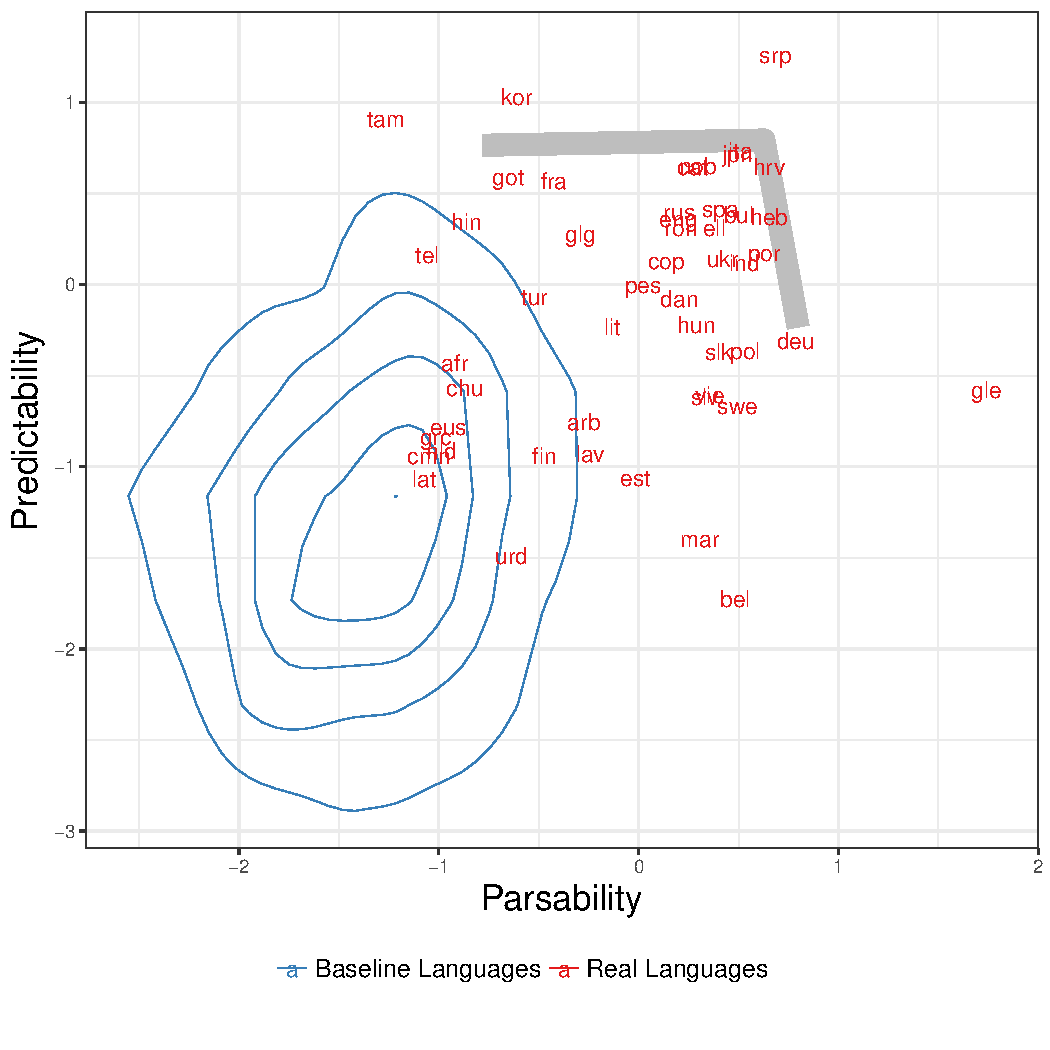
\includegraphics[scale=.45]{../results/plane/pareto-plane-iso-best-balanced-legend-viz-10.pdf}
    \caption{Predictability and parseability of 51 languages (red), indicated by ISO codes, compared to baseline word order grammars (blue distribution). Predictability and parseability scores are $z$-scored within language. The gray curve indicates the Pareto frontier of computationally optimized grammars, averaged over the 51 languages.} % TODO colors, fontsize, etc could conceivably be made prettier
    \label{fig:pareto-plane}
\end{figure}


\subsection{Greenbergian Word Order Correlations}
\label{sec:greenberg}

\begin{figure} % need Efficiency and (maybe) MLE langs on here
%	\includegraphics[width=0.3\textwidth]{../results/correlations/figures/coverage-ground_eff-circles.pdf}
	\begin{center}
	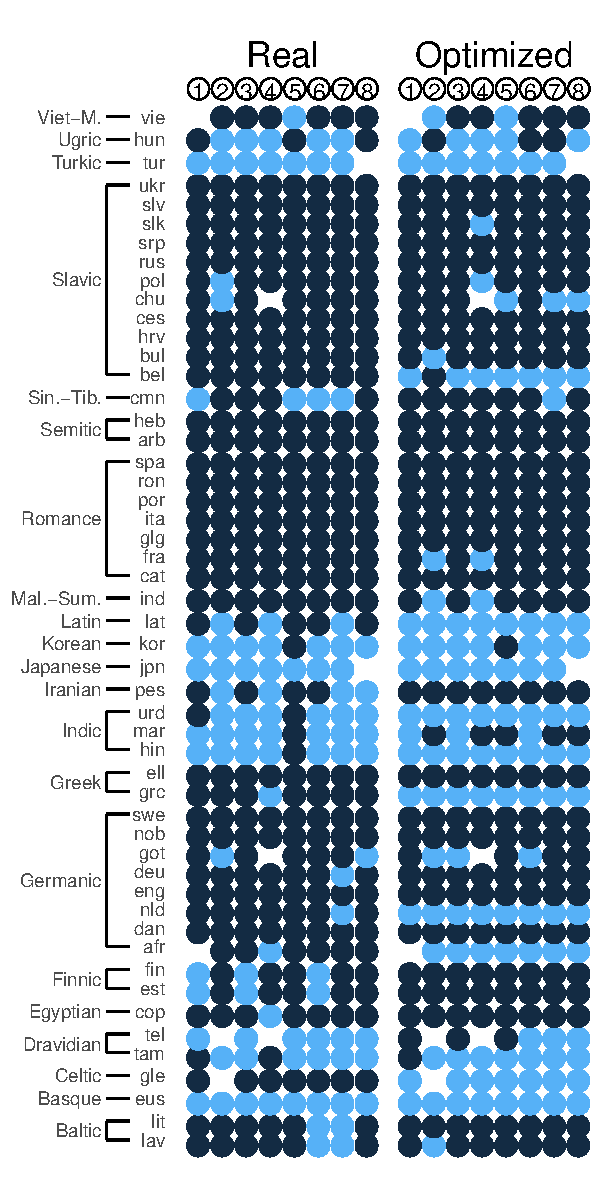
\includegraphics[width=0.32\textwidth]{../results/correlations/figures/pred-eff-families-2.pdf}
	\end{center}
	\caption{Order of the eight correlates across 51 languages, in the real grammars (left) and predicted by efficiency optimization (right). Dark blue: Verb patterner \emph{precedes} object patterner(English, Arabic, ...). Light blue: Verb patterner \emph{follows} object patterner (Japanese, Hindi , ...).}\label{fig:per-lang}
\end{figure}





\begin{table}
	\begin{center}
%		\setlength\tabcolsep{1.5pt}
\begin{tabular}{|c|ll|c|cc|ccc}
	\hline
	%&
	&	\multicolumn{2}{|c|}{Correlates with...}   &         \multirow{2}{*}{Real}   &  \multirow{2}{*}{Predicted} & \\ 
	&	verb & object     & & &   \\ 
	&	\emph{wrote} & \emph{letters} & & & \\ \hline \hline % \textsc{verb} $\xrightarrow{obj}$ \textsc{noun}
	\multirow{2}{*}{\raisebox{.5pt}{\textcircled{\raisebox{-.9pt} {1}}}}	&	adposition    &    NP       
				&   \multirow{2}{*}{  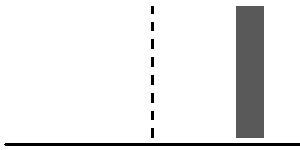
\includegraphics[width=0.06\textwidth]{../results/correlations/figures/posteriors/posterior_Real_lifted_case.pdf}     } 
		&   \multirow{2}{*}{  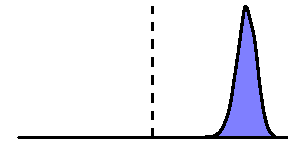
\includegraphics[width=0.06\textwidth]{../results/correlations/figures/posteriors/posterior_Efficiency_lifted_case.pdf}     } & \\
	&		\emph{to}            & \emph{a friend} &&&\\ \hline
	\multirow{2}{*}{\raisebox{.5pt}{\textcircled{\raisebox{-.9pt} {2}}}}	&copula    &    NP         
		&   \multirow{2}{*}{  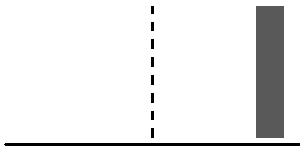
\includegraphics[width=0.06\textwidth]{../results/correlations/figures/posteriors/posterior_Real_lifted_cop.pdf}     } 
		&   \multirow{2}{*}{  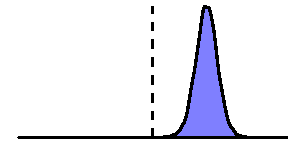
\includegraphics[width=0.06\textwidth]{../results/correlations/figures/posteriors/posterior_Efficiency_lifted_cop.pdf}     } & \\
	&	\emph{is}        & \emph{a friend}  &&&\\ \hline
	\multirow{2}{*}{\raisebox{.5pt}{\textcircled{\raisebox{-.9pt} {3}}}}	&auxiliary    &    VP       
		&   \multirow{2}{*}{  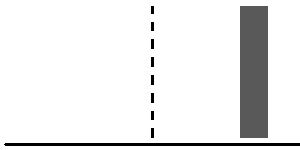
\includegraphics[width=0.06\textwidth]{../results/correlations/figures/posteriors/posterior_Real_aux.pdf}     } 
		&   \multirow{2}{*}{  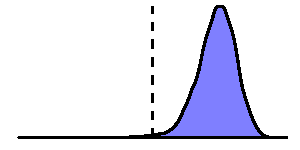
\includegraphics[width=0.06\textwidth]{../results/correlations/figures/posteriors/posterior_Efficiency_aux.pdf}     } & \\
	&	\emph{has}          & \emph{written}  &&&\\ \hline
	\multirow{2}{*}{\raisebox{.5pt}{\textcircled{\raisebox{-.9pt} {4}}}}	&noun    &    genitive      
		&   \multirow{2}{*}{  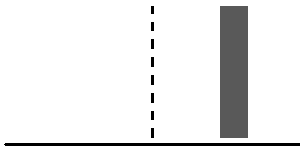
\includegraphics[width=0.06\textwidth]{../results/correlations/figures/posteriors/posterior_Real_nmod.pdf}     } 
		&   \multirow{2}{*}{  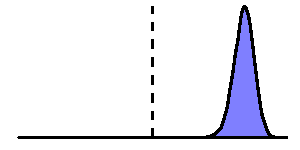
\includegraphics[width=0.06\textwidth]{../results/correlations/figures/posteriors/posterior_Efficiency_nmod.pdf}     } & \\
	&	\emph{friend} &  \emph{of John}  &&&\\ \hline
	\multirow{2}{*}{\raisebox{.5pt}{\textcircled{\raisebox{-.9pt} {5}}}}	&noun    &    relative clause      
		&   \multirow{2}{*}{  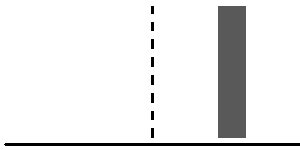
\includegraphics[width=0.06\textwidth]{../results/correlations/figures/posteriors/posterior_Real_acl.pdf}     } 
		&   \multirow{2}{*}{  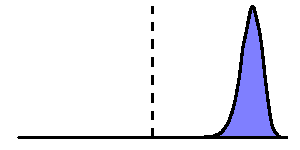
\includegraphics[width=0.06\textwidth]{../results/correlations/figures/posteriors/posterior_Efficiency_acl.pdf}     } & \\
	&	\emph{books} & \emph{that you read}  &&&\\ \hline
	\multirow{2}{*}{\raisebox{.5pt}{\textcircled{\raisebox{-.9pt} {6}}}}	&complementizer    &    S        
		&   \multirow{2}{*}{  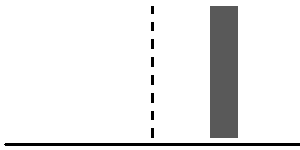
\includegraphics[width=0.06\textwidth]{../results/correlations/figures/posteriors/posterior_Real_lifted_mark.pdf}     } 
		&   \multirow{2}{*}{  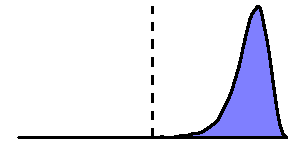
\includegraphics[width=0.06\textwidth]{../results/correlations/figures/posteriors/posterior_Efficiency_lifted_mark.pdf}     } & \\
	&	\emph{that} & \emph{she has arrived}  &&&\\ \hline
	\multirow{2}{*}{	\raisebox{.5pt}{\textcircled{\raisebox{-.9pt} {7}}}}	&verb    &    PP         
		&   \multirow{2}{*}{  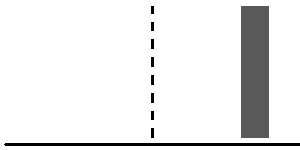
\includegraphics[width=0.06\textwidth]{../results/correlations/figures/posteriors/posterior_Real_obl.pdf}     } 
		&   \multirow{2}{*}{  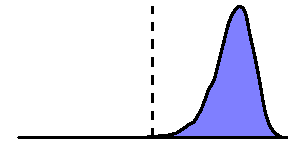
\includegraphics[width=0.06\textwidth]{../results/correlations/figures/posteriors/posterior_Efficiency_obl.pdf}     } & \\
	&	\emph{went} & \emph{to school}  &&&\\ \hline
	\multirow{2}{*}{\raisebox{.5pt}{\textcircled{\raisebox{-.9pt} {8}}}}	&want    &    VP        
		&   \multirow{2}{*}{  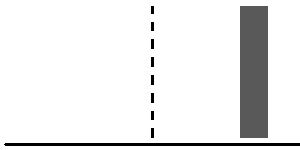
\includegraphics[width=0.06\textwidth]{../results/correlations/figures/posteriors/posterior_Real_xcomp.pdf}     } 
		&   \multirow{2}{*}{  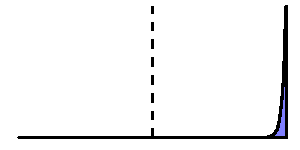
\includegraphics[width=0.06\textwidth]{../results/correlations/figures/posteriors/posterior_Efficiency_xcomp.pdf}     } & \\
	& \emph{wants}   &  \emph{to leave}  &&&\\ \hline
 \hline
%comp. &
%\multirow{3}{*}{NP}&
%	AP &
%    \multicolumn{4}{l}{\footnotesize{Significance levels: $^*$: $p < 0.05$, : $p < 0.01$, : $p < 0.001$}}
\end{tabular}
	\end{center}
\caption{Efficiency optimization accurately predicts the Greenbergian correlations.
For each correlation, we provide the distribution among the actual grammars of the 51 languages (left), and among grammars optimized for efficiency (right).
Efficiency optimization predicts all eight correlations to hold in the majority of grammars.
}\label{table:corr-resu}
\end{table}
















We now show that this process of efficiency optimization accounts for Greenberg's correlation universals. % we examine the computatinally optimized grammars. %computationally construct grammars that optimize efficiency, and evaluate these for dependency length and for Greenberg's universals.
For every one of the 51 languages, we create hypothetical grammars that are computationally optimized for efficiency (see \textit{Materials and Methods}).
In all results reported here, we set $\lambda := 0.9$ in Equation~\ref{eq:efficiency}.
(See SI appendix section 5 for mathematical justification and for robustness to other choices).
We test whether the process of efficiency optimization can explain these typological patterns, and make correct predictions about the orderings used in individual languages. %, this shows that efficiency optimization predicts Greenberg's word order correlation universals.



We compare grammars optimized for efficiency with the actual grammars of the 51 languages, as extracted from the orderings attested in the original corpora and validated against expert judgments (see \textit{Materials and Methods}).

We first evaluated which of the eight correlations emerge from efficiency optimization across language families.
We controlled for variation across different optima by creating eight optimized grammars for each language.
We controlled for variation between languages and language families by constructing a single Bayesian mixed-effects logistic regression model predicting which correlations an optimized grammar satisfies, entering the language and language family as random effects.
In this analysis, efficiency optimization predicts all eight correlations to hold across languages with posterior probability $0.9911$. 

In Table~\ref{table:corr-resu}, we compare the prevalence of the eight correlations in real and optimized languages.
For the real languages, we indicate how many of the 51 languages satisfy a correlation.
For the optimized languages, we indicate the posterior distribution of the proportion of satisfying languages, obtained from the mixed-effects analysis (see \textit{Materials and Methods}).
Grammars optimized for efficiency accurately predict all eight correlations to hold at prevalences significantly greater than 50\%, similar to actual human languages.
Optimizing for only predicability or only parseability does not predict all of the correlations (see SI).




We confirmed these results by evaluating predictions of efficiency optimization on the level of individual laguages (Figure~\ref{fig:per-lang}).
For every one of the 51 languages, we show orders predicted by efficiency, for the eight correlating pairs.
For each language, we consider the optimized grammar that had the best efficiency value, among those with the direction of the verb-object relation fixed to correspond to the actual language.
Predictions of efficiency optimization agree with the actual word order patterns in 82~\% of the cases.
Note that perfect agreement is not to be expected, as grammars will be impacted by factors other than efficiency optimization, such as their historical development.
For instance, Dutch (nld) and Afrikaans (afr) have a prevalence of object-verb order in corpus data, and efficiency optimization accordingly predicts them to have corresponding orders (light blue).
However, Dutch and Afrikaans have orders similar to the other Germanic languages (dark blue), which they are historically closely related to.






We have directly implemented parseability and predictability using general-purpose statistical models of language and dependency structures.
Prior work has considered Dependency Length Minimization (DLM) as an approximate formalization of efficiency optimization~\cite{futrell2015largescale,liu2017dependency,temperley2018minimizing}.
This is the idea that languages order words so as to minimize the overall length of dependencies.
This principle is a heuristic formalization of the idea that long dependencies should create high memory requirements in parsing and prediction~\cite{hawkins1994performance,gibson1998linguistic,gibson2000dependency, futrell2017memory}.
Indeed, directly modeling efficiency optimization predicts DLM, and appears to predict word order universals with greater accuracy than optimizing for DLM (see SI, \emph{Relation to Dependency Length Minimization}).






\section{Conclusion}

We found that a large subset of the Greenbergian word order correlations can be explained in terms of optimization of grammars for efficient communication, as defined by information theoretic criteria and implemented using state-of-the-art machine learning methods. We defined a space of word order grammars, as well as objective functions reflecting communicative efficiency, and found that the word order grammars that maximize communicative efficiency reproduce the word order universals. Beyond our present results, we provide a complete formalization and computational framework in which theories of the functional optimization of languages can be tested. Other objective functions could be hypothesized and tested within our framework; furthermore, future advances in machine learning will enable the optimization of richer and richer models of grammar.

A major question for functional explanations for linguistic universals is: \emph{how} do languages come to be optimized? Do speakers actively seek out new communicative conventions that allow better efficiency? Or do languages change in response to biases that come into play during language acquisition \cite{fedzechkina2012language,culbertson2012learning}? Our work is neutral toward such questions. To the extent that language universals arise from biases in learning or in the representational capacity of the human brain, our results suggest that those biases tilt toward communicative efficiency. Our work does provide evidence against the idea that word order universals are best explained in terms of learning biases that are irreducibly arbitrary and genetic in nature \cite{chomsky2010some}.

While our work has shown that certain word order universals can be explained by efficiency in communication, we have made a number of basic assumptions about how language works in constructing our word order grammars: for example, that sentences can be syntactically analyzed into dependency trees. The question arises of whether these more basic properties themselves might be explainable in terms of efficient communication. Relatedly, there are  remaining word order universals not captured by our model, such as the trade-off of rich morphological marking and flexibility in word order \cite{jespersen1922,mcfadden2003morphological,futrell2015quantifying}. Our models cannot capture this trade-off for technical reasons: the parseability objective does not operate over wordforms, only POS tags, and so it does not take advantage of morphological cues to syntactic structure. Future work can investigate whether these and other remaining universals can be explained using more sophisticated models of how meaning representations are transduced into strings of words, based on larger databases with richer annotations.




\matmethods{We base our experiments on the Universal Dependencies 2.1 treebanks~\cite{nivre2017universal}. % \footnote{\url{http://universaldependencies.org/}}
We use all languages for which at least one treebank with a training partition was available, a total of 51 languages.
For each language where multiple treebanks with training sets were available, we pooled their training sets; similarly for development sets.
Punctuation was removed.
%We removed punctuation. %, which we operationalized by removing all dependents of \emph{punct} dependencies, and recursively removing their dependents.

Universal dependencies represents as dependents some words that are typically classified as heads in syntactic theory.
This particularly applies to the \textit{cc}, \textit{case}, \textit{cop}, and \textit{mark} dependencies.
Following prior work studying dependency length minimization \cite{futrell2015largescale}, we modified each treebank by inverting these dependencies, promoting the dependent to the head position.
We report results on this modified version of UD.

The efficiency optimization results from Table~\ref{tab:results-dryer} were preregistered: \url{http://aspredicted.org/blind.php?x=8gp2bt}.

Code and results are available at \url{https://github.com/m-hahn/grammar-optim}.

See the SI for details on the neural language models and parsers used, and on the optimization procedures.}



\showmatmethods{} % Display the Materials and Methods section

%\acknow{We thank Ted Gibson, Michael C. Frank, Judith Degen, Noah Goodman, Chris Manning, and audiences at CAMP 2018 and CUNY 2019 for helpful discussion.}

\showacknow{} % Display the acknowledgments section


%\bibliographystyle{acl_natbib}
%\bibliography{extracted}
\bibliography{everything}


\end{document}









%%
%%
%
%\begin{table}
%	\begin{center}
%%		\setlength\tabcolsep{1.5pt}
%\begin{tabular}{c|ll|c|cc|ccc}
%	\hline
%	%&
%	&	\multicolumn{2}{|c|}{Correlates with...}   &         \multirow{2}{*}{Real}   &  \multirow{2}{*}{Predicted} & \\ 
%	&	verb & object     & & &   \\ 
%	&	\emph{wrote} & \emph{letters} & & & \\ \hline \hline % \textsc{verb} $\xrightarrow{obj}$ \textsc{noun}
%	\multirow{2}{*}{\raisebox{.5pt}{\textcircled{\raisebox{-.9pt} {1}}}}	&	adposition    &    NP       
%		& \multirow{2}{*}{\includegraphics[width=0.03\textwidth]{../results/correlations/figures/correlations/bars-ground-lifted_case.pdf} } %\textbf{86}  }
%	%	&   \multirow{2}{*}{ \includegraphics[width=0.03\textwidth]{../results/correlations/figures/correlations/bars-depl-lifted_case.pdf}       }
%	%	&    \multirow{2}{*}{\includegraphics[width=0.03\textwidth]{../results/correlations/figures/correlations/bars-langmod-lifted_case.pdf} } %  \textbf{47 \%}$^{}$   }
%	%	&    \multirow{2}{*}{\includegraphics[width=0.03\textwidth]{../results/correlations/figures/correlations/bars-parser-lifted_case.pdf}   }   
%		&   \multirow{2}{*}{  \includegraphics[width=0.03\textwidth]{../results/correlations/figures/correlations/bars-efficiency_large_best-lifted_case.pdf}     } & \\
%	&		\emph{to}            & \emph{a friend} &&&\\ \hline
%	\multirow{2}{*}{\raisebox{.5pt}{\textcircled{\raisebox{-.9pt} {2}}}}	&copula    &    NP         
%		&  \multirow{2}{*}{\includegraphics[width=0.03\textwidth]{../results/correlations/figures/correlations/bars-ground-lifted_cop.pdf} }% \textbf{94} }
%	%	&   \multirow{2}{*}{ \includegraphics[width=0.03\textwidth]{../results/correlations/figures/correlations/bars-depl-lifted_cop.pdf}       }
%	%	&    \multirow{2}{*}{\includegraphics[width=0.03\textwidth]{../results/correlations/figures/correlations/bars-langmod-lifted_cop.pdf} } % \textbf{53}     }
%	%	&   \multirow{2}{*}{  \includegraphics[width=0.03\textwidth]{../results/correlations/figures/correlations/bars-parser-lifted_cop.pdf}   }   
%		&   \multirow{2}{*}{  \includegraphics[width=0.03\textwidth]{../results/correlations/figures/correlations/bars-efficiency_large_best-lifted_cop.pdf}   } & \\
%	&	\emph{is}        & \emph{a friend}  &&&\\ \hline
%	\multirow{2}{*}{\raisebox{.5pt}{\textcircled{\raisebox{-.9pt} {3}}}}	&auxiliary    &    VP       
%		&  \multirow{2}{*}{\includegraphics[width=0.03\textwidth]{../results/correlations/figures/correlations/bars-ground-aux.pdf}}
%	%	&   \multirow{2}{*}{ \includegraphics[width=0.03\textwidth]{../results/correlations/figures/correlations/bars-depl-aux.pdf}       }
%	%	&    \multirow{2}{*}{\includegraphics[width=0.03\textwidth]{../results/correlations/figures/correlations/bars-langmod-aux.pdf}     }
%	%	&   \multirow{2}{*}{ \includegraphics[width=0.03\textwidth]{../results/correlations/figures/correlations/bars-parser-aux.pdf}  }   
%		&   \multirow{2}{*}{  \includegraphics[width=0.03\textwidth]{../results/correlations/figures/correlations/bars-efficiency_large_best-aux.pdf}  } & \\
%	&	\emph{has}          & \emph{written}  &&&\\ \hline
%	\multirow{2}{*}{\raisebox{.5pt}{\textcircled{\raisebox{-.9pt} {4}}}}	&noun    &    genitive      
%		&  \multirow{2}{*}{\includegraphics[width=0.03\textwidth]{../results/correlations/figures/correlations/bars-ground-nmod.pdf}}
%	%	&   \multirow{2}{*}{ \includegraphics[width=0.03\textwidth]{../results/correlations/figures/correlations/bars-depl-nmod.pdf}     }
%	%	&    \multirow{2}{*}{\includegraphics[width=0.03\textwidth]{../results/correlations/figures/correlations/bars-langmod-nmod.pdf}   }
%	%	&   \multirow{2}{*}{ \includegraphics[width=0.03\textwidth]{../results/correlations/figures/correlations/bars-parser-nmod.pdf}  }   
%		&   \multirow{2}{*}{  \includegraphics[width=0.03\textwidth]{../results/correlations/figures/correlations/bars-efficiency_large_best-nmod.pdf}  } & \\
%	&	\emph{friend} &  \emph{of John}  &&&\\ \hline
%	\multirow{2}{*}{\raisebox{.5pt}{\textcircled{\raisebox{-.9pt} {5}}}}	&noun    &    relative clause      
%		&  \multirow{2}{*}{\includegraphics[width=0.03\textwidth]{../results/correlations/figures/correlations/bars-ground-acl.pdf}}
%	%	&   \multirow{2}{*}{  \includegraphics[width=0.03\textwidth]{../results/correlations/figures/correlations/bars-depl-acl.pdf}     }
%	%	&    \multirow{2}{*}{\includegraphics[width=0.03\textwidth]{../results/correlations/figures/correlations/bars-langmod-acl.pdf}   }
%	%	&   \multirow{2}{*}{ \includegraphics[width=0.03\textwidth]{../results/correlations/figures/correlations/bars-parser-acl.pdf}  }   
%		&   \multirow{2}{*}{  \includegraphics[width=0.03\textwidth]{../results/correlations/figures/correlations/bars-efficiency_large_best-acl.pdf}  } & \\
%	&	\emph{books} & \emph{that you read}  &&&\\ \hline
%	\multirow{2}{*}{\raisebox{.5pt}{\textcircled{\raisebox{-.9pt} {6}}}}	&complementizer    &    S        
%		&  \multirow{2}{*}{\includegraphics[width=0.03\textwidth]{../results/correlations/figures/correlations/bars-ground-lifted_mark.pdf}}
%	%	&   \multirow{2}{*}{ \includegraphics[width=0.03\textwidth]{../results/correlations/figures/correlations/bars-depl-lifted_mark.pdf}     }
%	%	&    \multirow{2}{*}{\includegraphics[width=0.03\textwidth]{../results/correlations/figures/correlations/bars-langmod-lifted_mark.pdf}     }
%	%	&   \multirow{2}{*}{  \includegraphics[width=0.03\textwidth]{../results/correlations/figures/correlations/bars-parser-lifted_mark.pdf} }   
%		&   \multirow{2}{*}{  \includegraphics[width=0.03\textwidth]{../results/correlations/figures/correlations/bars-efficiency_large_best-lifted_mark.pdf}  }  &\\
%	&	\emph{that} & \emph{she has arrived}  &&&\\ \hline
%	\multirow{2}{*}{	\raisebox{.5pt}{\textcircled{\raisebox{-.9pt} {7}}}}	&verb    &    PP         
%		&  \multirow{2}{*}{\includegraphics[width=0.03\textwidth]{../results/correlations/figures/correlations/bars-ground-obl.pdf}}
%	%	&   \multirow{2}{*}{ \includegraphics[width=0.03\textwidth]{../results/correlations/figures/correlations/bars-depl-obl.pdf}     }
%	%	&    \multirow{2}{*}{\includegraphics[width=0.03\textwidth]{../results/correlations/figures/correlations/bars-langmod-obl.pdf}     }
%	%	&   \multirow{2}{*}{  \includegraphics[width=0.03\textwidth]{../results/correlations/figures/correlations/bars-parser-obl.pdf} }   
%		&   \multirow{2}{*}{  \includegraphics[width=0.03\textwidth]{../results/correlations/figures/correlations/bars-efficiency_large_best-obl.pdf}  } &  \\
%	&	\emph{went} & \emph{to school}  &&&\\ \hline
%	\multirow{2}{*}{\raisebox{.5pt}{\textcircled{\raisebox{-.9pt} {8}}}}	&want    &    VP        
%		&  \multirow{2}{*}{\includegraphics[width=0.03\textwidth]{../results/correlations/figures/correlations/bars-ground-xcomp.pdf}}
%	%	&   \multirow{2}{*}{ \includegraphics[width=0.03\textwidth]{../results/correlations/figures/correlations/bars-depl-nmod.pdf}     }
%	%	&    \multirow{2}{*}{\includegraphics[width=0.03\textwidth]{../results/correlations/figures/correlations/bars-langmod-xcomp.pdf}     }
%	%	&   \multirow{2}{*}{ \includegraphics[width=0.03\textwidth]{../results/correlations/figures/correlations/bars-parser-nmod.pdf}  }   
%		&   \multirow{2}{*}{  \includegraphics[width=0.03\textwidth]{../results/correlations/figures/correlations/bars-efficiency_large_best-xcomp.pdf}  } & \\
%	& \emph{wants}   &  \emph{to leave}  &&&\\ \hline
% \hline
%%comp. &
%%\multirow{3}{*}{NP}&
%%	AP &
%%    \multicolumn{4}{l}{\footnotesize{Significance levels: $^*$: $p < 0.05$, : $p < 0.01$, : $p < 0.001$}}
%\end{tabular}
%	\end{center}
%\caption{OPTION 1: Efficiency optimization accurately predicts the Greenbergian correlations. Each correlation is stated in terms of a pair of a `verb patterner' and an `object patterner', whose relative order correlate with that of verbs and objects.
%For each correlation, we provide an English example, and show the distribution among the actual grammars of the 51 languages (left), and among grammars optimized for efficiency (right).
%Blue bars count grammars conforming to the correlation, red bars count grammars violating it.
%Efficiency optimization predicts all eight correlations to hold in the majority of grammars.
%%Given the statistical nature of the correlations, not every language satisfies every one of them.
%%Not all correlations are satisfied by every natu
%}\label{table:corr-dryer}
%\end{table}
%






%
%\begin{table}
%	\begin{center}
%%		\setlength\tabcolsep{1.5pt}
%\begin{tabular}{|ll|c|cc|}
%	\hline
%	%&
%	\multicolumn{2}{|c|}{Correlates with...}   &         \multirow{2}{*}{Real}   & \multirow{2}{*}{DepL}  &  \multirow{2}{*}{Eff}  \\ 
%	verb & object     & & &   \\ \hline \hline % \textsc{verb} $\xrightarrow{obj}$ \textsc{noun}
%%adp. &
%	adposition    &    NP       
%	& \multirow{2}{*}{\includegraphics[width=0.05\textwidth]{../results/correlations/figures/correlations/correlation-ground-lifted_case.pdf} } %\textbf{86}  }
%%	&   \multirow{2}{*}{ \includegraphics[width=0.05\textwidth]{../results/correlations/figures/correlations/correlation-depl-lifted_case.pdf}       }
%%	&    \multirow{2}{*}{\includegraphics[width=0.05\textwidth]{../results/correlations/figures/correlations/correlation-langmod-lifted_case.pdf} } %  \textbf{47 \%}$^{}$   }
%%	&    \multirow{2}{*}{\includegraphics[width=0.05\textwidth]{../results/correlations/figures/correlations/correlation-parser-lifted_case.pdf}   }   
%	&   \multirow{2}{*}{  \includegraphics[width=0.05\textwidth]{../results/correlations/figures/correlations/correlation-efficiency-lifted_case.pdf}     }  \\
%	\emph{to}            & \emph{a friend} &&&\\ \hline
%copula    &    NP         
%	&  \multirow{2}{*}{\includegraphics[width=0.05\textwidth]{../results/correlations/figures/correlations/correlation-ground-lifted_cop.pdf} }% \textbf{94} }
%%	&   \multirow{2}{*}{ \includegraphics[width=0.05\textwidth]{../results/correlations/figures/correlations/correlation-depl-lifted_cop.pdf}       }
%%	&    \multirow{2}{*}{\includegraphics[width=0.05\textwidth]{../results/correlations/figures/correlations/correlation-langmod-lifted_cop.pdf} } % \textbf{53}     }
%%	&   \multirow{2}{*}{  \includegraphics[width=0.05\textwidth]{../results/correlations/figures/correlations/correlation-parser-lifted_cop.pdf}   }   
%	&   \multirow{2}{*}{  \includegraphics[width=0.05\textwidth]{../results/correlations/figures/correlations/correlation-efficiency-lifted_cop.pdf}   }  \\
%	\emph{is}        & \emph{a friend}  &&&\\ \hline
%auxiliary    &    VP       
%	&  \multirow{2}{*}{\includegraphics[width=0.05\textwidth]{../results/correlations/figures/correlations/correlation-ground-aux.pdf}}
%%	&   \multirow{2}{*}{ \includegraphics[width=0.05\textwidth]{../results/correlations/figures/correlations/correlation-depl-aux.pdf}       }
%%	&    \multirow{2}{*}{\includegraphics[width=0.05\textwidth]{../results/correlations/figures/correlations/correlation-langmod-aux.pdf}     }
%%	&   \multirow{2}{*}{ \includegraphics[width=0.05\textwidth]{../results/correlations/figures/correlations/correlation-parser-aux.pdf}  }   
%	&   \multirow{2}{*}{  \includegraphics[width=0.05\textwidth]{../results/correlations/figures/correlations/correlation-efficiency-aux.pdf}  }  \\
%	\emph{has}          & \emph{written}  &&&\\ \hline
%noun    &    genitive      
%	&  \multirow{2}{*}{\includegraphics[width=0.05\textwidth]{../results/correlations/figures/correlations/correlation-ground-nmod.pdf}}
%%	&   \multirow{2}{*}{ \includegraphics[width=0.05\textwidth]{../results/correlations/figures/correlations/correlation-depl-nmod.pdf}     }
%%	&    \multirow{2}{*}{\includegraphics[width=0.05\textwidth]{../results/correlations/figures/correlations/correlation-langmod-nmod.pdf}   }
%%	&   \multirow{2}{*}{ \includegraphics[width=0.05\textwidth]{../results/correlations/figures/correlations/correlation-parser-nmod.pdf}  }   
%	&   \multirow{2}{*}{  \includegraphics[width=0.05\textwidth]{../results/correlations/figures/correlations/correlation-efficiency-nmod.pdf}  }  \\
%	\emph{friend} &  \emph{of John}  &&&\\ \hline
%noun    &    relative clause      
%	&  \multirow{2}{*}{\includegraphics[width=0.05\textwidth]{../results/correlations/figures/correlations/correlation-ground-acl.pdf}}
%%	&   \multirow{2}{*}{  \includegraphics[width=0.05\textwidth]{../results/correlations/figures/correlations/correlation-depl-acl.pdf}     }
%%	&    \multirow{2}{*}{\includegraphics[width=0.05\textwidth]{../results/correlations/figures/correlations/correlation-langmod-acl.pdf}   }
%%	&   \multirow{2}{*}{ \includegraphics[width=0.05\textwidth]{../results/correlations/figures/correlations/correlation-parser-acl.pdf}  }   
%	&   \multirow{2}{*}{  \includegraphics[width=0.05\textwidth]{../results/correlations/figures/correlations/correlation-efficiency-acl.pdf}  }  \\
%	\emph{books} & \emph{that you read}  &&&\\ \hline
%complementizer    &    S        
%	&  \multirow{2}{*}{\includegraphics[width=0.05\textwidth]{../results/correlations/figures/correlations/correlation-ground-lifted_mark.pdf}}
%%	&   \multirow{2}{*}{ \includegraphics[width=0.05\textwidth]{../results/correlations/figures/correlations/correlation-depl-lifted_mark.pdf}     }
%%	&    \multirow{2}{*}{\includegraphics[width=0.05\textwidth]{../results/correlations/figures/correlations/correlation-langmod-lifted_mark.pdf}     }
%%	&   \multirow{2}{*}{  \includegraphics[width=0.05\textwidth]{../results/correlations/figures/correlations/correlation-parser-lifted_mark.pdf} }   
%	&   \multirow{2}{*}{  \includegraphics[width=0.05\textwidth]{../results/correlations/figures/correlations/correlation-efficiency-lifted_mark.pdf}  }  \\
%	\emph{that} & \emph{she has arrived}  &&&\\ \hline
%verb    &    PP         
%	&  \multirow{2}{*}{\includegraphics[width=0.05\textwidth]{../results/correlations/figures/correlations/correlation-ground-obl.pdf}}
%%	&   \multirow{2}{*}{ \includegraphics[width=0.05\textwidth]{../results/correlations/figures/correlations/correlation-depl-obl.pdf}     }
%%	&    \multirow{2}{*}{\includegraphics[width=0.05\textwidth]{../results/correlations/figures/correlations/correlation-langmod-obl.pdf}     }
%%	&   \multirow{2}{*}{  \includegraphics[width=0.05\textwidth]{../results/correlations/figures/correlations/correlation-parser-obl.pdf} }   
%	&   \multirow{2}{*}{  \includegraphics[width=0.05\textwidth]{../results/correlations/figures/correlations/correlation-efficiency-obl.pdf}  }  \\
%	\emph{went} & \emph{to school}  &&&\\ \hline
%want    &    VP        
%	&  \multirow{2}{*}{\includegraphics[width=0.05\textwidth]{../results/correlations/figures/correlations/correlation-ground-xcomp.pdf}}
%%	&   \multirow{2}{*}{ \includegraphics[width=0.05\textwidth]{../results/correlations/figures/correlations/correlation-depl-nmod.pdf}     }
%%	&    \multirow{2}{*}{\includegraphics[width=0.05\textwidth]{../results/correlations/figures/correlations/correlation-langmod-xcomp.pdf}     }
%%	&   \multirow{2}{*}{ \includegraphics[width=0.05\textwidth]{../results/correlations/figures/correlations/correlation-parser-nmod.pdf}  }   
%	&   \parbox[c]{0.05\textwidth}{\multirow{2}{*}{  \includegraphics[width=0.05\textwidth]{../results/correlations/figures/correlations/correlation-efficiency-xcomp.pdf}  }}  \\
%	\emph{wants}   &  \emph{to leave}  &&&\\ \hline
% \hline
%%comp. &
%%\multirow{3}{*}{NP}&
%%	AP &
%    \multicolumn{4}{l}{\footnotesize{Significance levels: $^*$: $p < 0.05$, : $p < 0.01$, : $p < 0.001$}}
%\end{tabular}
%	\end{center}
%	\caption{Greenbergian Correlations. Each correlation is stated in terms of a pair of a `verb patterner' and an `object patterner', whose relative order correlate with that of verbs and objects.
%For each correlation, we provide an English example, and show the distribution of real languages, of languages optimized for DLM, and of languages optimized for efficiency. The process of optimization fir efficiency and DLM explains all eight universals.
%%Given the statistical nature of the correlations, not every language satisfies every one of them.
%%Not all correlations are satisfied by every natu
%}\label{table:corr-dryer}
%\end{table}
%
%

%
%
%\begin{table}
%	\begin{center}
%%		\setlength\tabcolsep{1.5pt}
%\begin{tabular}{|ll|c|cc|cc|}
%	\hline
%	%&
%	\multicolumn{2}{|c|}{Correlates with...}   &         \multirow{2}{*}{Real}   & \multirow{2}{*}{DepL}  &  \multirow{2}{*}{Parser}  &  \multirow{2}{*}{Eff}  \\ 
%	verb & object     & & &   \\ \hline \hline % \textsc{verb} $\xrightarrow{obj}$ \textsc{noun}
%%adp. &
%	adposition    &    NP       
%	& \multirow{2}{*}{\includegraphics[width=0.03\textwidth]{../results/correlations/figures/correlations/bars-ground-lifted_case.pdf} } %\textbf{86}  }
%	&   \multirow{2}{*}{ \includegraphics[width=0.03\textwidth]{../results/correlations/figures/correlations/bars-depl-lifted_case.pdf}       }
%%	&    \multirow{2}{*}{\includegraphics[width=0.03\textwidth]{../results/correlations/figures/correlations/bars-langmod-lifted_case.pdf} } %  \textbf{47 \%}$^{}$   }
%	&    \multirow{2}{*}{\includegraphics[width=0.03\textwidth]{../results/correlations/figures/correlations/bars-parser-lifted_case.pdf}   }   
%	&   \multirow{2}{*}{  \includegraphics[width=0.03\textwidth]{../results/correlations/figures/correlations/bars-efficiency_large_best-lifted_case.pdf}     }  \\
%	\emph{to}            & \emph{a friend} &&&\\ \hline
%copula    &    NP         
%	&  \multirow{2}{*}{\includegraphics[width=0.03\textwidth]{../results/correlations/figures/correlations/bars-ground-lifted_cop.pdf} }% \textbf{94} }
%	&   \multirow{2}{*}{ \includegraphics[width=0.03\textwidth]{../results/correlations/figures/correlations/bars-depl-lifted_cop.pdf}       }
%%	&    \multirow{2}{*}{\includegraphics[width=0.03\textwidth]{../results/correlations/figures/correlations/bars-langmod-lifted_cop.pdf} } % \textbf{53}     }
%	&   \multirow{2}{*}{  \includegraphics[width=0.03\textwidth]{../results/correlations/figures/correlations/bars-parser-lifted_cop.pdf}   }   
%	&   \multirow{2}{*}{  \includegraphics[width=0.03\textwidth]{../results/correlations/figures/correlations/bars-efficiency_large_best-lifted_cop.pdf}   }  \\
%	\emph{is}        & \emph{a friend}  &&&\\ \hline
%auxiliary    &    VP       
%	&  \multirow{2}{*}{\includegraphics[width=0.03\textwidth]{../results/correlations/figures/correlations/bars-ground-aux.pdf}}
%	&   \multirow{2}{*}{ \includegraphics[width=0.03\textwidth]{../results/correlations/figures/correlations/bars-depl-aux.pdf}       }
%%	&    \multirow{2}{*}{\includegraphics[width=0.03\textwidth]{../results/correlations/figures/correlations/bars-langmod-aux.pdf}     }
%	&   \multirow{2}{*}{ \includegraphics[width=0.03\textwidth]{../results/correlations/figures/correlations/bars-parser-aux.pdf}  }   
%	&   \multirow{2}{*}{  \includegraphics[width=0.03\textwidth]{../results/correlations/figures/correlations/bars-efficiency_large_best-aux.pdf}  }  \\
%	\emph{has}          & \emph{written}  &&&\\ \hline
%noun    &    genitive      
%	&  \multirow{2}{*}{\includegraphics[width=0.03\textwidth]{../results/correlations/figures/correlations/bars-ground-nmod.pdf}}
%	&   \multirow{2}{*}{ \includegraphics[width=0.03\textwidth]{../results/correlations/figures/correlations/bars-depl-nmod.pdf}     }
%%	&    \multirow{2}{*}{\includegraphics[width=0.03\textwidth]{../results/correlations/figures/correlations/bars-langmod-nmod.pdf}   }
%	&   \multirow{2}{*}{ \includegraphics[width=0.03\textwidth]{../results/correlations/figures/correlations/bars-parser-nmod.pdf}  }   
%	&   \multirow{2}{*}{  \includegraphics[width=0.03\textwidth]{../results/correlations/figures/correlations/bars-efficiency_large_best-nmod.pdf}  }  \\
%	\emph{friend} &  \emph{of John}  &&&\\ \hline
%noun    &    relative clause      
%	&  \multirow{2}{*}{\includegraphics[width=0.03\textwidth]{../results/correlations/figures/correlations/bars-ground-acl.pdf}}
%	&   \multirow{2}{*}{  \includegraphics[width=0.03\textwidth]{../results/correlations/figures/correlations/bars-depl-acl.pdf}     }
%%	&    \multirow{2}{*}{\includegraphics[width=0.03\textwidth]{../results/correlations/figures/correlations/bars-langmod-acl.pdf}   }
%	&   \multirow{2}{*}{ \includegraphics[width=0.03\textwidth]{../results/correlations/figures/correlations/bars-parser-acl.pdf}  }   
%	&   \multirow{2}{*}{  \includegraphics[width=0.03\textwidth]{../results/correlations/figures/correlations/bars-efficiency_large_best-acl.pdf}  }  \\
%	\emph{books} & \emph{that you read}  &&&\\ \hline
%complementizer    &    S        
%	&  \multirow{2}{*}{\includegraphics[width=0.03\textwidth]{../results/correlations/figures/correlations/bars-ground-lifted_mark.pdf}}
%	&   \multirow{2}{*}{ \includegraphics[width=0.03\textwidth]{../results/correlations/figures/correlations/bars-depl-lifted_mark.pdf}     }
%%	&    \multirow{2}{*}{\includegraphics[width=0.03\textwidth]{../results/correlations/figures/correlations/bars-langmod-lifted_mark.pdf}     }
%	&   \multirow{2}{*}{  \includegraphics[width=0.03\textwidth]{../results/correlations/figures/correlations/bars-parser-lifted_mark.pdf} }   
%	&   \multirow{2}{*}{  \includegraphics[width=0.03\textwidth]{../results/correlations/figures/correlations/bars-efficiency_large_best-lifted_mark.pdf}  }  \\
%	\emph{that} & \emph{she has arrived}  &&&\\ \hline
%verb    &    PP         
%	&  \multirow{2}{*}{\includegraphics[width=0.03\textwidth]{../results/correlations/figures/correlations/bars-ground-obl.pdf}}
%	&   \multirow{2}{*}{ \includegraphics[width=0.03\textwidth]{../results/correlations/figures/correlations/bars-depl-obl.pdf}     }
%%	&    \multirow{2}{*}{\includegraphics[width=0.03\textwidth]{../results/correlations/figures/correlations/bars-langmod-obl.pdf}     }
%	&   \multirow{2}{*}{  \includegraphics[width=0.03\textwidth]{../results/correlations/figures/correlations/bars-parser-obl.pdf} }   
%	&   \multirow{2}{*}{  \includegraphics[width=0.03\textwidth]{../results/correlations/figures/correlations/bars-efficiency_large_best-obl.pdf}  }  \\
%	\emph{went} & \emph{to school}  &&&\\ \hline
%want    &    VP        
%	&  \multirow{2}{*}{\includegraphics[width=0.03\textwidth]{../results/correlations/figures/correlations/bars-ground-xcomp.pdf}}
%	&   \multirow{2}{*}{ \includegraphics[width=0.03\textwidth]{../results/correlations/figures/correlations/bars-depl-nmod.pdf}     }
%%	&    \multirow{2}{*}{\includegraphics[width=0.03\textwidth]{../results/correlations/figures/correlations/bars-langmod-xcomp.pdf}     }
%	&   \multirow{2}{*}{ \includegraphics[width=0.03\textwidth]{../results/correlations/figures/correlations/bars-parser-nmod.pdf}  }   
%	&   \multirow{2}{*}{  \includegraphics[width=0.03\textwidth]{../results/correlations/figures/correlations/bars-efficiency_large_best-xcomp.pdf}  }  \\
%	\emph{wants}   &  \emph{to leave}  &&&\\ \hline
% \hline
%%comp. &
%%\multirow{3}{*}{NP}&
%%	AP &
%    \multicolumn{4}{l}{\footnotesize{Significance levels: $^*$: $p < 0.05$, : $p < 0.01$, : $p < 0.001$}}
%\end{tabular}
%	\end{center}
%	\caption{Greenbergian Correlations. Each correlation is stated in terms of a pair of a `verb patterner' and an `object patterner', whose relative order correlate with that of verbs and objects.
%For each correlation, we provide an English example, and show the distribution of real languages, of languages optimized for DLM, and of languages optimized for efficiency. The process of optimization fir efficiency and DLM explains all eight universals.
%%Given the statistical nature of the correlations, not every language satisfies every one of them.
%%Not all correlations are satisfied by every natu
%}\label{table:corr-dryer}
%\end{table}
%
%





%\begin{table*}
%	\begin{center}
%\begin{tabular}{|ll|l|l|l|ll|l|}
%	\hline
%	%&
%	\multicolumn{2}{|c|}{Correlates with...}   &         \multirow{2}{*}{Real}   & \multirow{2}{*}{DepL}  & \multirow{2}{*}{Pred}   &  \multirow{2}{*}{Pars} &  \multirow{2}{*}{Efficiency}  \\ 
%	verb & object     & & & &  & \\ \hline \hline % \textsc{verb} $\xrightarrow{obj}$ \textsc{noun}
%%adp. &
%adposition    &    NP       &    86    &    \textbf{81}$^{***}$    &    47    &    \textbf{76}$^{***}$    &    \textbf{68}$^{***}$   \\
%copula    &    NP        &    94    &    \textbf{81}$^{***}$    &    53    &    \textbf{79}$^{***}$    &    \textbf{61}$^{**}$   \\
%auxiliary    &    VP       &    88    &    \textbf{74}$^{***}$    &    \textbf{84}$^{***}$    &    55    &    \textbf{69}$^{**}$   \\
%noun    &    genitive      &    80    &    \textbf{82}$^{***}$    &    55    &    \textbf{74}$^{***}$    &    \textbf{70}$^{***}$   \\
%noun    &    relative clause       &    80    &    \textbf{85}$^{***}$    &    48    &    \textbf{77}$^{**}$    &    \textbf{73}$^{***}$   \\
%complementizer    &    S        &    76    &    \textbf{85}$^{***}$    &    \textbf{59}$^{**}$    &    \textbf{80}$^{***}$    &    \textbf{74}$^{**}$   \\
%verb    &    PP     &    88    &    \textbf{78}$^{***}$    &    \textbf{72}$^{***}$    &    59    &    \textbf{69}$^{**}$   \\
%want    &    VP      &    88    &    \textbf{90}$^{***}$    &    \textbf{78}$^{**}$    &    \textbf{92}$^{***}$    &    \textbf{92}$^{***}$   \\
%verb    &    subject    &    33    &    \textbf{29}$^{**}$    &    51    &    \textbf{8}$^{***}$    &    \textbf{13}$^{***}$   \\
%verb    &    manner adverb     &    35    &    51    &    \textbf{21}$^{***}$    &    51    &    \textbf{32}$^{***}$   \\
% \hline
%%comp. &
%%\multirow{3}{*}{NP}&
%%	AP &
%    \multicolumn{6}{l}{\footnotesize{Significance levels: $^*$: $p < 0.05$, $^{**}$: $p < 0.01$, $^{***}$: $p < 0.001$}}
%\end{tabular}
%	\end{center}
%	\caption{Greenbergian Correlations. Following \cite{dryer1992greenbergian}, each correlation is stated in terms of a pair of a `verb patterner' and an `object patterner', whose relative order correlate with that of verbs and objects.
%%	For clarity, we organize the correlations by the category of the `verb patterner'.
%	For each correlation, we give our operationalization in terms of UD. %A rightwards arrow indicates that the dependency is predicted to have the same direction as the \textit{obj} dependency; a leftwards arrow indicates an inverse correlation. 
%	For each correlation we report what percentage of the languages in our sample satisfied it (`Real').
%	We then report, for each correlation and each objective function, how many (in \%) of the optimized grammars satisfy the correlation, with the significance level in a logistic mixed-effects analysis across language families.}\label{table:results-dryer}
%\end{table*}
%



%We show that Efficiency optimization predicts DLM, providing a first-principles functional explanation.
%%Functional studies of word order have proposed Dependency Length Minimization (DLM) as general principle of word order \cite{futrell2015largescale,liu2017dependency,temperley2018minimizing}.
%Figure~\ref{fig:deplength} shows average dependency length for real languages, random baselines, and languages optimized for dependency length and efficiency.
%Optimizing for efficiency lowers dependency length relative to random baselines.

%It has also been argued theoretically that this principle should account for Greenberg's correlations, though this link is nontrivial and depends on the precise distributions of tree topologies in syntactic structures.
%As a principle of word order, DLM is stipulative: There are other processing models, such as surprisal, that are strongly predictive of human processing cost, and make predictions distinct from, and partly conflicting with, those of DLM~\cite{hale2001probabilistic,levy2008expectation}.
%\cite{futrell2017memory} suggests that efficiency predicts DLM.


%Our results suggest that dependency length minimization is a by-product of efficiency maximization. In 80\% of the languages, optimizing explicitly for dependency length produces dependencies that overshoot the dependency length of the real language; on average, the real language is best matched by efficiency optimization.

%\begin{figure} % need Efficiency and (maybe) MLE langs on here
%\includegraphics[width=0.4\textwidth]{../results/dependency-length/figures/depl-violin.pdf}
%	\caption{Average dependency length for real languages (blue), random baselines (purple), and for languages optimized for efficiency (green) and explicitly for dependency length (red). Dependency length was computed from sentences of lengths 8-12 and averaged over words.}\label{fig:deplength}
%\end{figure}








\begin{table}
	\begin{center}
%		\setlength\tabcolsep{1.5pt}
\begin{tabular}{|c|ll|c|cc|ccc}
	\hline
	%&
	&	\multicolumn{2}{|c|}{Correlates with...}   &         \multirow{2}{*}{Real}   &  \multirow{2}{*}{Predicted} & \\ 
	&	verb & object     & & &   \\ 
	&	\emph{wrote} & \emph{letters} & & & \\ \hline \hline % \textsc{verb} $\xrightarrow{obj}$ \textsc{noun}
	\multirow{2}{*}{\raisebox{.5pt}{\textcircled{\raisebox{-.9pt} {1}}}}	&	adposition    &    NP       
				&   \multirow{2}{*}{  \includegraphics[width=0.06\textwidth]{../results/correlations/figures/posteriors/posterior_Real_lifted_case.pdf}     } 
		&   \multirow{2}{*}{  \includegraphics[width=0.06\textwidth]{../results/correlations/figures/posteriors/posterior_Efficiency_lifted_case.pdf}     } & \\
	&		\emph{to}            & \emph{a friend} &&&\\ \hline
	\multirow{2}{*}{\raisebox{.5pt}{\textcircled{\raisebox{-.9pt} {2}}}}	&copula    &    NP         
		&   \multirow{2}{*}{  \includegraphics[width=0.06\textwidth]{../results/correlations/figures/posteriors/posterior_Real_lifted_cop.pdf}     } 
		&   \multirow{2}{*}{  \includegraphics[width=0.06\textwidth]{../results/correlations/figures/posteriors/posterior_Efficiency_lifted_cop.pdf}     } & \\
	&	\emph{is}        & \emph{a friend}  &&&\\ \hline
	\multirow{2}{*}{\raisebox{.5pt}{\textcircled{\raisebox{-.9pt} {3}}}}	&auxiliary    &    VP       
		&   \multirow{2}{*}{  \includegraphics[width=0.06\textwidth]{../results/correlations/figures/posteriors/posterior_Real_aux.pdf}     } 
		&   \multirow{2}{*}{  \includegraphics[width=0.06\textwidth]{../results/correlations/figures/posteriors/posterior_Efficiency_aux.pdf}     } & \\
	&	\emph{has}          & \emph{written}  &&&\\ \hline
	\multirow{2}{*}{\raisebox{.5pt}{\textcircled{\raisebox{-.9pt} {4}}}}	&noun    &    genitive      
		&   \multirow{2}{*}{  \includegraphics[width=0.06\textwidth]{../results/correlations/figures/posteriors/posterior_Real_nmod.pdf}     } 
		&   \multirow{2}{*}{  \includegraphics[width=0.06\textwidth]{../results/correlations/figures/posteriors/posterior_Efficiency_nmod.pdf}     } & \\
	&	\emph{friend} &  \emph{of John}  &&&\\ \hline
	\multirow{2}{*}{\raisebox{.5pt}{\textcircled{\raisebox{-.9pt} {5}}}}	&noun    &    relative clause      
		&   \multirow{2}{*}{  \includegraphics[width=0.06\textwidth]{../results/correlations/figures/posteriors/posterior_Real_acl.pdf}     } 
		&   \multirow{2}{*}{  \includegraphics[width=0.06\textwidth]{../results/correlations/figures/posteriors/posterior_Efficiency_acl.pdf}     } & \\
	&	\emph{books} & \emph{that you read}  &&&\\ \hline
	\multirow{2}{*}{\raisebox{.5pt}{\textcircled{\raisebox{-.9pt} {6}}}}	&complementizer    &    S        
		&   \multirow{2}{*}{  \includegraphics[width=0.06\textwidth]{../results/correlations/figures/posteriors/posterior_Real_lifted_mark.pdf}     } 
		&   \multirow{2}{*}{  \includegraphics[width=0.06\textwidth]{../results/correlations/figures/posteriors/posterior_Efficiency_lifted_mark.pdf}     } & \\
	&	\emph{that} & \emph{she has arrived}  &&&\\ \hline
	\multirow{2}{*}{	\raisebox{.5pt}{\textcircled{\raisebox{-.9pt} {7}}}}	&verb    &    PP         
		&   \multirow{2}{*}{  \includegraphics[width=0.06\textwidth]{../results/correlations/figures/posteriors/posterior_Real_obl.pdf}     } 
		&   \multirow{2}{*}{  \includegraphics[width=0.06\textwidth]{../results/correlations/figures/posteriors/posterior_Efficiency_obl.pdf}     } & \\
	&	\emph{went} & \emph{to school}  &&&\\ \hline
	\multirow{2}{*}{\raisebox{.5pt}{\textcircled{\raisebox{-.9pt} {8}}}}	&want    &    VP        
		&   \multirow{2}{*}{  \includegraphics[width=0.06\textwidth]{../results/correlations/figures/posteriors/posterior_Real_xcomp.pdf}     } 
		&   \multirow{2}{*}{  \includegraphics[width=0.06\textwidth]{../results/correlations/figures/posteriors/posterior_Efficiency_xcomp.pdf}     } & \\
	& \emph{wants}   &  \emph{to leave}  &&&\\ \hline
 \hline
%comp. &
%\multirow{3}{*}{NP}&
%	AP &
%    \multicolumn{4}{l}{\footnotesize{Significance levels: $^*$: $p < 0.05$, : $p < 0.01$, : $p < 0.001$}}
\end{tabular}
	\end{center}
\caption{OPTION 2: Efficiency optimization accurately predicts the Greenbergian correlations. Each correlation is stated in terms of a pair of a `verb patterner' and an `object patterner', whose relative order correlate with that of verbs and objects.
For each correlation, we provide an English example, and show the distribution among the actual grammars of the 51 languages (left), and among grammars optimized for efficiency (right).
Blue bars count grammars conforming to the correlation, red bars count grammars violating it.
Efficiency optimization predicts all eight correlations to hold in the majority of grammars.
%Given the statistical nature of the correlations, not every language satisfies every one of them.
%Not all correlations are satisfied by every natu
}\label{table:corr-dryer}
\end{table}








\begin{table}
	\begin{center}
%		\setlength\tabcolsep{1.5pt}
\begin{tabular}{c|ll|c|cc|ccc}
	\hline
	%&
	&	\multicolumn{2}{|c|}{Correlates with...}   &         \multirow{2}{*}{Real}   &  \multirow{2}{*}{Predicted} & \\ 
	&	verb & object     & & &   \\ 
	&	\emph{wrote} & \emph{letters} & & & \\ \hline \hline % \textsc{verb} $\xrightarrow{obj}$ \textsc{noun}
	\multirow{2}{*}{\raisebox{.5pt}{\textcircled{\raisebox{-.9pt} {1}}}}	&	adposition    &    NP       
				&   \multirow{2}{*}{  \includegraphics[width=0.06\textwidth]{../results/correlations/figures/posteriors/posterior_Real_lifted_case.pdf}     } 
		&    & \\
	&		\emph{to}            & \emph{a friend} &&&\\ 
	&&& {  \includegraphics[width=0.06\textwidth]{../results/correlations/figures/posteriors/posterior_Efficiency_lifted_case.pdf}     } \\ \hline
	\multirow{2}{*}{\raisebox{.5pt}{\textcircled{\raisebox{-.9pt} {2}}}}	&copula    &    NP         
		&   \multirow{2}{*}{  \includegraphics[width=0.06\textwidth]{../results/correlations/figures/posteriors/posterior_Real_lifted_cop.pdf}     } 
	%	&   \multirow{2}{*}{ \includegraphics[width=0.03\textwidth]{../results/correlations/figures/correlations/bars-depl-lifted_cop.pdf}       }
	%	&    \multirow{2}{*}{\includegraphics[width=0.03\textwidth]{../results/correlations/figures/correlations/bars-langmod-lifted_cop.pdf} } % \textbf{53}     }
	%	&   \multirow{2}{*}{  \includegraphics[width=0.03\textwidth]{../results/correlations/figures/correlations/bars-parser-lifted_cop.pdf}   }   
		& & \\
	&	\emph{is}        & \emph{a friend}  &&&\\ 
	&&&   {  \includegraphics[width=0.06\textwidth]{../results/correlations/figures/posteriors/posterior_Efficiency_lifted_cop.pdf}     } \\ \hline
	\multirow{2}{*}{\raisebox{.5pt}{\textcircled{\raisebox{-.9pt} {3}}}}	&auxiliary    &    VP       
		&   \multirow{2}{*}{  \includegraphics[width=0.06\textwidth]{../results/correlations/figures/posteriors/posterior_Real_aux.pdf}     } 
	%	&   \multirow{2}{*}{ \includegraphics[width=0.03\textwidth]{../results/correlations/figures/correlations/bars-depl-aux.pdf}       }
	%	&    \multirow{2}{*}{\includegraphics[width=0.03\textwidth]{../results/correlations/figures/correlations/bars-langmod-aux.pdf}     }
	%	&   \multirow{2}{*}{ \includegraphics[width=0.03\textwidth]{../results/correlations/figures/correlations/bars-parser-aux.pdf}  }   
		&  & \\
	&	\emph{has}          & \emph{written}  &&&\\ 
	&&&  {  \includegraphics[width=0.06\textwidth]{../results/correlations/figures/posteriors/posterior_Efficiency_aux.pdf}     } \\ \hline
	\multirow{2}{*}{\raisebox{.5pt}{\textcircled{\raisebox{-.9pt} {4}}}}	&noun    &    genitive      
		&   \multirow{2}{*}{  \includegraphics[width=0.06\textwidth]{../results/correlations/figures/posteriors/posterior_Real_nmod.pdf}     } 
	%	&   \multirow{2}{*}{ \includegraphics[width=0.03\textwidth]{../results/correlations/figures/correlations/bars-depl-nmod.pdf}     }
	%	&    \multirow{2}{*}{\includegraphics[width=0.03\textwidth]{../results/correlations/figures/correlations/bars-langmod-nmod.pdf}   }
	%	&   \multirow{2}{*}{ \includegraphics[width=0.03\textwidth]{../results/correlations/figures/correlations/bars-parser-nmod.pdf}  }   
		&   \multirow{2}{*}{  \includegraphics[width=0.06\textwidth]{../results/correlations/figures/posteriors/posterior_Efficiency_nmod.pdf}     } & \\
	&	\emph{friend} &  \emph{of John}  &&&\\ \hline
	\multirow{2}{*}{\raisebox{.5pt}{\textcircled{\raisebox{-.9pt} {5}}}}	&noun    &    relative clause      
		&   \multirow{2}{*}{  \includegraphics[width=0.06\textwidth]{../results/correlations/figures/posteriors/posterior_Real_acl.pdf}     } 
	%	&   \multirow{2}{*}{  \includegraphics[width=0.03\textwidth]{../results/correlations/figures/correlations/bars-depl-acl.pdf}     }
	%	&    \multirow{2}{*}{\includegraphics[width=0.03\textwidth]{../results/correlations/figures/correlations/bars-langmod-acl.pdf}   }
	%	&   \multirow{2}{*}{ \includegraphics[width=0.03\textwidth]{../results/correlations/figures/correlations/bars-parser-acl.pdf}  }   
		&   \multirow{2}{*}{  \includegraphics[width=0.06\textwidth]{../results/correlations/figures/posteriors/posterior_Efficiency_acl.pdf}     } & \\
	&	\emph{books} & \emph{that you read}  &&&\\ \hline
	\multirow{2}{*}{\raisebox{.5pt}{\textcircled{\raisebox{-.9pt} {6}}}}	&complementizer    &    S        
		&   \multirow{2}{*}{  \includegraphics[width=0.06\textwidth]{../results/correlations/figures/posteriors/posterior_Real_lifted_mark.pdf}     } 
	%	&   \multirow{2}{*}{ \includegraphics[width=0.03\textwidth]{../results/correlations/figures/correlations/bars-depl-lifted_mark.pdf}     }
	%	&    \multirow{2}{*}{\includegraphics[width=0.03\textwidth]{../results/correlations/figures/correlations/bars-langmod-lifted_mark.pdf}     }
	%	&   \multirow{2}{*}{  \includegraphics[width=0.03\textwidth]{../results/correlations/figures/correlations/bars-parser-lifted_mark.pdf} }   
		&   \multirow{2}{*}{  \includegraphics[width=0.06\textwidth]{../results/correlations/figures/posteriors/posterior_Efficiency_lifted_mark.pdf}     } & \\
	&	\emph{that} & \emph{she has arrived}  &&&\\ \hline
	\multirow{2}{*}{	\raisebox{.5pt}{\textcircled{\raisebox{-.9pt} {7}}}}	&verb    &    PP         
		&   \multirow{2}{*}{  \includegraphics[width=0.06\textwidth]{../results/correlations/figures/posteriors/posterior_Real_obl.pdf}     } 
	%	&   \multirow{2}{*}{ \includegraphics[width=0.03\textwidth]{../results/correlations/figures/correlations/bars-depl-obl.pdf}     }
	%	&    \multirow{2}{*}{\includegraphics[width=0.03\textwidth]{../results/correlations/figures/correlations/bars-langmod-obl.pdf}     }
	%	&   \multirow{2}{*}{  \includegraphics[width=0.03\textwidth]{../results/correlations/figures/correlations/bars-parser-obl.pdf} }   
		&   \multirow{2}{*}{  \includegraphics[width=0.06\textwidth]{../results/correlations/figures/posteriors/posterior_Efficiency_obl.pdf}     } & \\
	&	\emph{went} & \emph{to school}  &&&\\ \hline
	\multirow{2}{*}{\raisebox{.5pt}{\textcircled{\raisebox{-.9pt} {8}}}}	&want    &    VP        
		&   \multirow{2}{*}{  \includegraphics[width=0.06\textwidth]{../results/correlations/figures/posteriors/posterior_Real_xcomp.pdf}     } 
	%	&   \multirow{2}{*}{ \includegraphics[width=0.03\textwidth]{../results/correlations/figures/correlations/bars-depl-nmod.pdf}     }
	%	&    \multirow{2}{*}{\includegraphics[width=0.03\textwidth]{../results/correlations/figures/correlations/bars-langmod-xcomp.pdf}     }
	%	&   \multirow{2}{*}{ \includegraphics[width=0.03\textwidth]{../results/correlations/figures/correlations/bars-parser-nmod.pdf}  }   
		&   \multirow{2}{*}{  \includegraphics[width=0.06\textwidth]{../results/correlations/figures/posteriors/posterior_Efficiency_xcomp.pdf}     } & \\
	& \emph{wants}   &  \emph{to leave}  &&&\\ \hline
 \hline
%comp. &
%\multirow{3}{*}{NP}&
%	AP &
%    \multicolumn{4}{l}{\footnotesize{Significance levels: $^*$: $p < 0.05$, : $p < 0.01$, : $p < 0.001$}}
\end{tabular}
	\end{center}
\caption{OPTION 2: Efficiency optimization accurately predicts the Greenbergian correlations. Each correlation is stated in terms of a pair of a `verb patterner' and an `object patterner', whose relative order correlate with that of verbs and objects.
For each correlation, we provide an English example, and show the distribution among the actual grammars of the 51 languages (left), and among grammars optimized for efficiency (right).
Blue bars count grammars conforming to the correlation, red bars count grammars violating it.
Efficiency optimization predicts all eight correlations to hold in the majority of grammars.
%Given the statistical nature of the correlations, not every language satisfies every one of them.
%Not all correlations are satisfied by every natu
}\label{table:corr-dryer}
\end{table}



%the meaning



\begin{figure}
\centering
\begin{dependency}[theme = simple]
   \begin{deptext}[column sep=1em]
%	   I \& wrote \& the \& letter \& in \& Japanese \& . \\
	   katabt \& risāla \& li \& sadīq  \\
	   \textsc{verb} \& \textsc{noun} \& \textsc{adp} \& \textsc{noun} \\
	   wrote \& letter   \& to \& friend  \\
   \end{deptext}
\end{dependency}
\begin{dependency}[theme = simple]
   \begin{deptext}[column sep=1em]
      tomodachi \& ni \& tegami-o \& kaita \\
 \textsc{noun} \& \textsc{adp} \& \textsc{noun} \& \textsc{verb}\\
	   friend \& to \& letter  \& wrote \\
   \end{deptext}
\end{dependency}

%\begin{dependency}[theme=simple]
%    \begin{deptext}
%    I \& wrote \& a \& letter \& to \& a \& friend \\
%    \end{deptext}
%    \depedge{2}{1}{nsubj}
%    \depedge{2}{4}{obj}
%    \depedge{4}{3}{ }
%    \depedge{4}{3}{ }
%    \depedge{2}{5}{}
%    \depedge{5}{7}{ }
%    \depedge{7}{6}{ }
%\end{dependency}
	\caption{A sentence in Arabic (top) and Japanese (bottom), translating to `I wrote a letter to a friend.' Note the reversal of word order: Arabic has verb-object order and prepositions, while Japanese has object-verb order and postpositions.}\label{fig:arabic-japanese-simple}
\end{figure}



\section{Minimizing Dependency Length Predicts Universals}


..


\begin{figure}
\centering
\begin{dependency}[theme = simple]
   \begin{deptext}[column sep=1em]
%	   I \& wrote \& the \& letter \& in \& Japanese \& . \\
	   katabt \& risāla \& li \& sadīq  \\
	   \textsc{verb} \& \textsc{noun} \& \textsc{adp} \& \textsc{noun} \\
	   wrote \& letter   \& to \& friend  \\
   \end{deptext}
	%   \deproot{3}{ROOT}
   \depedge{1}{2}{obj}
	%   \depedge[edge start x offset=-6pt]{2}{5}{ATT}
   \depedge{1}{3}{}
   \depedge{3}{4}{}
   %\depedge[arc angle=50]{7}{6}{ATT}
\end{dependency}
\begin{dependency}[theme = simple]
   \begin{deptext}[column sep=1em]
      tomodachi \& ni \& tegami-o \& kaita \\
 \textsc{noun} \& \textsc{adp} \& \textsc{noun} \& \textsc{verb}\\
	   friend \& to \& letter  \& wrote \\
   \end{deptext}
	%   \deproot{3}{ROOT}
   \depedge{4}{2}{}
	%   \depedge[edge start x offset=-6pt]{2}{5}{ATT}
   \depedge{2}{1}{}
   \depedge{4}{3}{obj}
   %\depedge[arc angle=50]{7}{6}{ATT}
\end{dependency}
\end{figure}





Dependency Length:


The sentences in Figure~\ref{fig:arabic-japanese} are annotated with \key{dependency trees}: these are directed trees describing the grammatical relations among words. For example, the arcs labeled ``obj'' represent that the noun in question is the \emph{direct object} if the verb, rather than e.g. the subject or an indirect object. A dependency arc is drawn from a \key{head} (e.g. \emph{kaita} in Figure~\ref{fig:arabic-japanese}) to a \key{dependent} (e.g. \emph{tegami-o}). Dependency trees can be defined in terms of many different syntactic theories \cite{corbett1993heads}. Although there are some differences in how different formalisms would draw trees for certain sentences, there is broad enough agreement about dependency trees that it has been possible to develop large-scale dependency-annotated corpora of text from dozens of languages \cite{nivre2017universal}.

In order to interpret a sentence correctly, a listener must be able to reconstruct the information expressed in the dependency tree and its labels. This is because, according to the principle of compositionality \cite{frege1892sinn}, the meaning of a sentence is a function of the meanings of the parts and how they are combined; the dependency tree (including the labels on the arcs) specifies how the meanings of words are combined.




The contribution of this work is (i) to provide a principled formalization of the notion of communicative efficiency in word order, based on related work in information theory \cite{cover2006elements,tishby1999information}, bounded rationality \cite{genewein2015bounded}, and computational neuroscience \cite{friston2009predictive}; (ii) to introduce a computational framework in which we can produce simulated grammars directly optimized for our notion of efficiency, using state-of-the-art machine learning techniques \cite{hochreiter1997long,goldberg2017neural,dozat2017stanford}; and (iii) to demonstrate that in doing so, we reproduce the major word order patterns reported in \cite{greenberg1963universals} and related work \cite{dryer1992greenbergian}, as well as reproducing the predictions of previous heuristic theories of word order optimization \cite{hawkins1994performance,ferrericancho2004euclidean,liu2008dependency,gildea2010grammars,futrell2015largescale}.

We formalize the notion of communicative efficiency using two terms: one having to do with minimizing the difficulty of linguistic communication, and one having to do with maximizing the information transferred in such communication. We quantify the difficulty of linguistic communication in terms of the word-by-word \key{predictability} of strings, which has been found to be a highly accurate and general predictor of human online comprehension difficulty \cite{hale2001probabilistic,levy2008expectation,smith2013effect}, and which can be justified in terms of predictive coding theories of information processing in the brain \cite{friston2009predictive} as well as the general algorithmic complexity of language generation and comprehension \cite{li2008introduction}. We quantify the information transferred in language as \key{parseability}: the quantity of information linguistic utterances contain about latent hierarchical tree structures. We also compare the results of optimizing for communicative efficiency to the results of optimizing for dependency length minimization, a previously proposed approximate metric of the amount of memory involved in language production and comprehension \cite{hudson1995measuring,gibson1998linguistic,gibson2000dependency,liu2017dependency,temperley2018minimizing}.

To evaluate whether communicative efficiency can explain word order universals, we apply the following method \cite{gildea2007optimizing}. First, we develop word order grammars: simple, interpretable models of word order, implemented as functions that take in an unordered syntactic dependency tree and output a distribution over possible word orders for that tree. Second, we take dependency treebanks of natural languages and compute word order grammars which are optimized for an objective functions representing communicative efficiency.
Third, we evaluate whether the optimized word order grammars reproduce the desired word order universals when applied to attested dependency trees from the treebanks across many languages. Our favorable results suggest that it may be possible to generally model human languages as efficient codes for communication among agents with generic human-like cognitive and communicative constraints. %The best way to describe a human language might be as a solution to an equation involving such constraints.

%We draw on data from the Universal Dependencies project \cite{nivre-universal-2017}, which has been developing treebanks in a unified format for several dozens of diverse languages.
%This universal annotation scheme is particularly useful for studying word order universals, as many of them can be operationalized  in terms of crosslinguistically valid syntactic notions. % such as \emph{verbs} and \emph{objects}.

\section{Background}


% TODO where do we say that we're basing our work on data from 51 languages?

%\subsection{Explananda: Word Order Correlations}
%
%Working with a database of 30 languages, Greenberg \cite{greenberg1963universals} proposed 45 universals of language that he determined to be true of most or all languages.
%31 of them were concerned with word order, the remainder with morphology.
%Many of the word order universals state \emph{correlations} between patterns:
%For instance, Universals 3 and 4 state that ``\emph{Languages with dominant VSO order are always prepositional.}''  (e.g. Arabic), and ``\emph{With overwhelmingly greater than chance frequency, languages with normal SOV order are postpositional.}'' (e.g. Japanese). 
%These are illustrated in Figure~\ref{fig:arabic-japanese}:
%Arabic has basic order verb-object (VO) and prepositions (\emph{li} `to'), while Japanese has order object-verb (OV) and postpositions (\emph{ni} `to'). Our goal is to explain Greenberg's reported word order correlations, as updated in \cite{dryer1992greenbergian}.

\begin{figure}
\centering
\begin{dependency}[theme = simple]
   \begin{deptext}[column sep=1em]
%	   I \& wrote \& the \& letter \& in \& Japanese \& . \\
	   katabt \& risāla \& li \& sadīq  \\
	   \textsc{verb} \& \textsc{noun} \& \textsc{adp} \& \textsc{noun} \\
	   wrote \& letter   \& to \& friend  \\
   \end{deptext}
	%   \deproot{3}{ROOT}
   \depedge{1}{2}{obj}
	%   \depedge[edge start x offset=-6pt]{2}{5}{ATT}
   \depedge{1}{3}{}
   \depedge{3}{4}{}
   %\depedge[arc angle=50]{7}{6}{ATT}
\end{dependency}
\begin{dependency}[theme = simple]
   \begin{deptext}[column sep=1em]
      tomodachi \& ni \& tegami-o \& kaita \\
 \textsc{noun} \& \textsc{adp} \& \textsc{noun} \& \textsc{verb}\\
	   friend \& to \& letter  \& wrote \\
   \end{deptext}
	%   \deproot{3}{ROOT}
   \depedge{4}{2}{}
	%   \depedge[edge start x offset=-6pt]{2}{5}{ATT}
   \depedge{2}{1}{}
   \depedge{4}{3}{obj}
   %\depedge[arc angle=50]{7}{6}{ATT}
\end{dependency}

%\begin{dependency}[theme=simple]
%    \begin{deptext}
%    I \& wrote \& a \& letter \& to \& a \& friend \\
%    \end{deptext}
%    \depedge{2}{1}{nsubj}
%    \depedge{2}{4}{obj}
%    \depedge{4}{3}{ }
%    \depedge{4}{3}{ }
%    \depedge{2}{5}{}
%    \depedge{5}{7}{ }
%    \depedge{7}{6}{ }
%\end{dependency}
	\caption{A sentence in Arabic (top) and Japanese (bottom), translating to `I wrote a letter to a friend.' Note the reversal of word order: Arabic has verb-object order and prepositions, while Japanese has object-verb order and postpositions.}\label{fig:arabic-japanese}
\end{figure}

% TODO what to do about these labels...? They're not UD...

\subsection{Dependency trees}

\section{Optimizing word order grammars}

Here we describe our model of word order and how we derive optimal grammars within that model in terms of communicative efficiency.

Let $t$ be an unordered dependency tree, i.e. a structure as in Figure~\ref{fig:arabic-japanese} but without any specified ordering of the words. We think of an unordered dependency tree $t$ as representing the compositional meaning to be conveyed by a sentence. We define a \key{word order grammar} as a function $L_\theta(t)$, whose behavior is specified by parameters $\theta$, which takes an unordered dependency tree $t$ as input and produces as output a probability distribution over ordered sequences of words $\mathbf{w}$ linearizing the tree, or equivalently, a probability distribution over orders on the nodes of the tree. % do we need to define "linearize"?
This process is visualized in Figure~\ref{fig:process-visualization}.

Next we define how a word order grammar linearizes trees in terms of its parameters $\theta$, and then we describe how $\theta$ can be set to optimize objective functions related to communicative efficiency.



\begin{figure}
\includegraphics[width=0.48\textwidth]{figures/process-visualization.png}
\caption{Our method for constructing counterfactual versions of languages: We extract unordered dependency tree topologies from dependency corpora, and apply word order grammars to obtain counterfactually reordered corpora.}\label{fig:process-visualization}
\end{figure}




We think of it as the following problem:

A speaker has a tree in mind, and they have to produce an utterance.



%Let $T$ be a distribution over unordered dependency trees and let $L_\theta$ be a word order grammar. Our goal is to find parameters $\theta$ which maximize an objective function $J$ in expectation over utterances:
%\begin{equation}
%\label{eq:exp-over-utts}
%J_T(\theta) = \E_{t \sim T} \E_{\mathbf{w} \sim L_\theta(t)} [R(t; \mathbf{w})], % TODO make the expectations look better!!
%\end{equation}
%where the function $R$ specifies a score for an individual utterance $\mathbf{w}$ expressing a tree $t$. In practice, $T$ will be the empirical distribution over unordered trees observed in a dependency treebank.
%Below we discuss possible values of $R$, which may implement predictability, parseability, or a weighted combination of the two, representing overall efficiency.
%
%

All natural languages have some degree of word order regularity. Thus, it is not sufficient to optimize the word orders of individual sentences in the corpora---instead, we will optimize the word order rules of entire languages.
We develop a method to create word order rules that optimize given processing measures on the resulting counterfactual corpus.

\subsection{DLM Predicts Universals}


We first apply our method to show that DLM predicts the correlations.



%Dependency length has been proposed as a metric of processing difficulty on the reasoning that long dependencies create high memory requirements for parsing and generation \cite{gibson1998linguistic,gibson2000dependency}, and minimization of dependency length is known to recover a large subset of the Greenbergian universals \cite{hawkins1994performance,hawkins2004efficiency,hawkins2014crosslinguistic}. 
%We demonstrate that the minimization of dependency length can be formalized in our framework, reproducing the finding that optimizing grammars for dependency length recovers several word order universals \cite{gildea2010grammars}.
%
%To quantify dependency length, we sum the lengths of syntactic dependencies in the sentence \cite{ferrericancho2004euclidean,liu2008dependency,gildea2010grammars,futrell2015largescale}:
%\begin{equation}
%    \label{eq:depl}
%	R_{DepL}(t; {\bf w}) = -\sum_{i=1}^{\# {\bf w}} |i - head(t; w_i)|,
%\end{equation}
%where $head(t; i) \in \{1, ..., n\}$ is the index of the head of $w_i$, and the sum is negative because dependency length is seen as a cost. 
Dependency length quantified in this manner is a heuristic measure of complexity: the actual processing complexity induced by long dependencies is not a linear function of length and depends crucially on the types of dependencies involved \cite{demberg2008data} and the specific elements intervening between the head and dependent \cite{gibson1998linguistic,gibson2000dependency,lewis2005activationbased}. 



\subsection{Efficiency Predicts Universals}


DLM is stipulative and at most a heuristic approximation to psycholinguistic findings


We now introduce a general information-theoretic notion of language efficiency.


use the general speaker-listener picture


\paragraph{Predictability}
Predictability represents the incremental difficulty of online language processing. We formalize predictability as the \key{surprisal} (negative log probability) of each word given its preceding context \cite{hale2001probabilistic,levy2008expectation,smith2013effect}. Optimization of predictability has been proposed as an explanation for certain word order patterns by \cite{ferrericancho2017optimality}.

We formalize predictability as follows. Given a language model $P_\phi$ with parameters $\phi$, the log probability of a sentence ${\bf w}$ is:
\begin{equation*}
R_{Pred}^\phi(t; {\bf w}) = \sum_{i=1}^{\#{\bf w}} \log P_\phi(w_{i+1}|w_{1\dots i}),
\end{equation*}
%where the language model parameters $\phi$ are chosen to predict the language induced by tree distribution $T$ and word order grammar $\L_\theta$ as accurately as possible (maximizing predictability):
%\begin{equation*}
%	\phi(\theta) = \argmax_\phi \displaystyle \E_{t \sim T} \E_{{\bf w} \sim L_\theta(t)} [ R^\phi_{Pred}({\bf w}, \phi) ].
%\end{equation*}
We implement the language model $P_\phi$ using an LSTM neural network architecture \cite{hochreiter1997long}, currently the state of the art for this task \cite{goldberg2017neural}.
%Note that the language model parameters $\phi$ and the word order grammar parameters $\theta$ are recursively dependent on each other.
See the SI for details on how $\theta$ and $\phi$ are jointly optimized, as well as on the neural network architecture.

\paragraph{Parseability}
Parseability is the extent to which the syntactic and semantic relationships among words can be recovered from the string of words. 
%Some notion of parseability has been proposed informally as a desirable property of languages in the linguistic literature going back at least to the 19th century \cite{humboldt,sapir,jesperson}, and parseability has been offered as an underlying justification for syntactic locality as a cost function for language processing \cite{hawkins-performance-1994}. 
%At a basic level, a language can encode information about syntactic relations into fixed word order patterns or into morphological marking on individual words. Much linguistic work has been devoted to investigating the trade-offs of various ways of indicating syntactic relations \cite{}. In this work, we present what is to our knowledge the first fully implemented computational formalization of this idea.
We specify parseability as the mutual information between strings and trees, or equivalently the quantity of information provided by strings about trees. Formally, we say the parseability score of an utterance $\mathbf{w}$ is the pointwise mutual information of the $\mathbf{w}$ and the tree $t$ it was generated from, calculated using a parser with parameters $\psi$:\footnote{Note that $P(t)$ is a constant term which will be ignored in the optimization process.}
\begin{align}
\nonumber
R_{Pars}^\psi(t; {\bf w}) &= \log \frac{P_\psi (t|\mathbf{w})}{P(t)} \\
\nonumber
&= \displaystyle \sum_{i=1}^{\#\mathbf{w}} \log P_\psi\left(\begin{array}{@{}l@{}}head(w_{i}) \\ label(w_i)\end{array}{\big |}\textbf{w}\right) - \log P(t),
\end{align}
%where the parser parameters $\psi$ are chosen to maximize parsing accuracy:
%\begin{equation*}
%\psi(\theta) = \argmax_\phi \displaystyle \E_{t \sim T} \E_{{\bf w} \sim L_\theta(t)} [ R_{Pars}({\bf w}, \psi) ].
%\end{equation*}
We implement $P_\psi$ using a highly generic graph-based parsing architecture \cite{kiperwasser2016simple,dozat2017stanford} which recovers graph structures from word strings by solving a minimal spanning tree problem.
%Due to data sparsity, we train parsers to predict dependency trees from POS tags alone, not from full wordforms, therefore we do not capture the extent to which morphological wordforms are informative about dependency tree structure.
See the SI (appendix section 6-7) for further details on the joint optimization of $\theta$ and $\psi$ and on the neural parser architecture, and see SI (section 8) for robustness to different parsing models.

\paragraph{Efficiency}
The two scoring functions---predictability and parseability---can be combined into an overall equation of the form:
\begin{equation}
\label{eq:combined-score}
	R_{\textit{Eff}} = R_{Pars} + \lambda R_{Pred},
\end{equation}
with an interpolation weight $\lambda \in [0,1)$. In all experiments in this paper we use $\lambda=.9$ (see SI appendix section 5 for mathematical justification). This combined equation represents efficiency: bits of information transferred about dependency trees minus the cost of the transmission. In expectation over utterances (substituting Eq.~\ref{eq:combined-score} into Eq.~\ref{eq:exp-over-utts}), the overall objective function to be maximized by a word order grammar can be written in information-theoretic terms as:
\begin{equation}
    \label{eq:efficiency}
    J_T(\theta) = I[L_\theta(T);T] - \lambda H[L_\theta(T)],
\end{equation}
where $I[L_\theta(T);T]$ is the \key{mutual information} between strings and trees, and $H[L_\theta(T)]$ is the \key{entropy} of strings \cite{cover2006elements}. Maximizing Eq.~\ref{eq:efficiency} is equivalent to maximizing mutual information between strings and trees subject to a constraint on the maximum entropy of strings. 

The two terms of Eq.~\ref{eq:efficiency} implement two opposing pressures. Parseability (the mutual information term) pushes to make strings more heterogeneous, so that they can indicate different tree structures unambiguously. Predictability (the entropy term) pushes to make strings more homogeneous, to reduce the complexity of using the language. The idea that natural language arises from a tension between these two forces goes back over a century \cite{gabelentz1901sprachwissenschaft}. Eq.~\ref{eq:efficiency} is a special case of the objective function proposed in \cite{ferrericancho2002zipf,ferrericancho2007global,futrell2017memory} as a general objective for communicative systems, taking unordered dependency trees $T$ as the underlying meanings to be conveyed. Eq.~\ref{eq:efficiency} can also be seen as a simplified form of the Information Bottleneck \cite{tishby1999information}, a general objective function for lossy compression which has recently been applied to explain linguistic phenomena such as color naming systems \cite{zaslavsky2018efficient} (see SI section 4 for the precise relationship). 




%In previous studies of word order optimization, it has been common to propose that word orders are chosen to minimize \key{dependency length}, the linear distance between words linked in head--dependent relationships \cite{futrell2015largescale,liu2017dependency,temperley2018minimizing}. 
\section{Results}

\subsection{Relative efficiency of languages}
\label{sec:relative-efficiency}

We first demonstrate that real languages are relatively efficient compared to random baselines. For each language, we generated ten baseline word order grammars for the language by choosing all word order grammar parameters randomly at uniform from $[0,1]$. Figure~\ref{fig:pareto-plane} shows the predictability and parseability for each real language relative to its baseline grammars. In order to control for limitations due to our word order grammar formalism, we represent real languages in the figure by maximum likelihood fits of word order grammars to the real language data.
%; in general these maximum-likelihood word order grammars end up with lower predictability and parseability than the real languages. % TODO verify this is true? TODO awkward sentence
For the calculation of predictability and parseability, we make all (baseline and real) word order grammars deterministic by always choosing the highest-probability linearization of each tree; by making the grammars deterministic in this way we eliminate an anticonservative bias toward low predictability in the baseline languages, which are highly nondeterministic. 
The majority of real languages in Figure~\ref{fig:pareto-plane} are below and to the left of their baseline equivalents, demonstrating that they are relatively high in predictability and/or parseability.

\begin{figure}
    \centering
    \includegraphics[scale=.45]{../results/plane/pareto-plane-iso-best-balanced-legend-viz.pdf}
    \caption{Predictability and parseability of 51 UD languages (red), indicated by ISO codes, compared to ten baseline word order grammars per language (green). Predictability and parseability scores are $z$-scored within language. Each point for a real language has a line pointing in the direction of the center of mass of its baselines. The green contour shows the density of baseline languages. Unlabeled dots represent the centroid for real languages (red), baseline languages (green), and languages optimized for predictability (yellow), parseability (pink), efficiency (blue), and dependency length (red). When a language is to the bottom--left of its baselines, this indicates that it is relatively optimal for efficiency.} % TODO colors, fontsize, etc could conceivably be made prettier
    \label{fig:pareto-plane}
\end{figure}

Figure~\ref{fig:pareto-plane} also shows the average position of optimized languages. Languages appear to be attracted toward these points and away from the region of the baseline languages. We also see that several languages actually end up \emph{more} efficient than the computationally optimized languages.
% TODO add something about dependency length-optimized languages?

These results are shown in more detail for two typologically distinct languages (English and Japanese) in Figure~\ref{fig:predict-pars}. Here we include also the predictability and parseability of the original language data and of the word order grammars optimized for dependency length. We see that real languages are even more predictable than any optimized or baseline language, while optimization for either parseability or dependency length suffices to raise parseability to the level of the real languages. This result is in line with the finding that languages with longer dependencies are harder to parse in general \cite{gulordava2016multilingual}.

\begin{figure*}
\includegraphics[width=0.98\textwidth]{../results/plot-by-lang/grid-optimized.pdf} % need MLE langs and Efficiency langs on here
	\caption{Predictability (top) and parseability (bottom) of real, optimized, and random languages, for English (left) and Japanese (right). We provide the entropy $H[L_\theta(T)]$ for predictability (lower is better) and the conditional entropy $H[T|L_\theta(T)]$ for parseability (lower is better). Both measures are normalized by sentence length.}\label{fig:predict-pars}
\end{figure*}

Finally we demonstrate the relationship between dependency length minimization and the maximization of efficiency. Figure~\ref{fig:deplength} shows average dependency length per sentence length for four typologically distinct languages, showing real languages, random baselines, and languages optimized for dependency length, parseability, predictability, and efficiency. We see that optimizing for efficiency lowers dependency length relative to random baselines, in keeping with the suggestion that dependency length minimization is a by-product of efficiency maximization \cite{futrell2017memory}. In 80\% of the languages, optimizing explicitly for dependency length produces dependencies that overshoot the depenndency length of the real language; in 3/4 of the lanuages shown, the real language is best matched by efficiency optimization.

\begin{figure*} % need Efficiency and (maybe) MLE langs on here
\includegraphics[width=0.98\textwidth]{../results/dependency-length/figures/depLength-facet.pdf}
\caption{Average dependency length as a function of sentence length in four languages. Across languages, real and optimized languages have shorter dependencies than random baseline orderings.}\label{fig:deplength}
\end{figure*}

\subsection{Greenbergian Word Order Correlations}
\label{sec:greenberg}
\begin{table*}
	\begin{center}
\begin{tabular}{|ll|l|l|l|ll|l|}
	\hline
	%&
	\multicolumn{2}{|c|}{Correlates with...}   &         \multirow{2}{*}{Real}   & \multirow{2}{*}{DepL}  & \multirow{2}{*}{Pred}   &  \multirow{2}{*}{Pars} &  \multirow{2}{*}{Efficiency}  \\ 
	verb & object     & & & &  & \\ \hline \hline % \textsc{verb} $\xrightarrow{obj}$ \textsc{noun}
%adp. &
adposition    &    NP       &    86    &    \textbf{81}$^{***}$    &    47    &    \textbf{76}$^{***}$    &    \textbf{68}$^{***}$   \\
copula    &    NP        &    94    &    \textbf{81}$^{***}$    &    53    &    \textbf{79}$^{***}$    &    \textbf{61}$^{**}$   \\
auxiliary    &    VP       &    88    &    \textbf{74}$^{***}$    &    \textbf{84}$^{***}$    &    55    &    \textbf{69}$^{**}$   \\
noun    &    genitive      &    80    &    \textbf{82}$^{***}$    &    55    &    \textbf{74}$^{***}$    &    \textbf{70}$^{***}$   \\
noun    &    relative clause       &    80    &    \textbf{85}$^{***}$    &    48    &    \textbf{77}$^{**}$    &    \textbf{73}$^{***}$   \\
complementizer    &    S        &    76    &    \textbf{85}$^{***}$    &    \textbf{59}$^{**}$    &    \textbf{80}$^{***}$    &    \textbf{74}$^{**}$   \\
verb    &    PP     &    88    &    \textbf{78}$^{***}$    &    \textbf{72}$^{***}$    &    59    &    \textbf{69}$^{**}$   \\
want    &    VP      &    88    &    \textbf{90}$^{***}$    &    \textbf{78}$^{**}$    &    \textbf{92}$^{***}$    &    \textbf{92}$^{***}$   \\
verb    &    subject    &    33    &    \textbf{29}$^{**}$    &    51    &    \textbf{8}$^{***}$    &    \textbf{13}$^{***}$   \\
verb    &    manner adverb     &    35    &    51    &    \textbf{21}$^{***}$    &    51    &    \textbf{32}$^{***}$   \\
 \hline
%comp. &
%\multirow{3}{*}{NP}&
%	AP &
    \multicolumn{6}{l}{\footnotesize{Significance levels: $^*$: $p < 0.05$, $^{**}$: $p < 0.01$, $^{***}$: $p < 0.001$}}
\end{tabular}
	\end{center}
	\caption{Greenbergian Correlations. Following \cite{dryer1992greenbergian}, each correlation is stated in terms of a pair of a `verb patterner' and an `object patterner', whose relative order correlate with that of verbs and objects.
%	For clarity, we organize the correlations by the category of the `verb patterner'.
	For each correlation, we give our operationalization in terms of UD. %A rightwards arrow indicates that the dependency is predicted to have the same direction as the \textit{obj} dependency; a leftwards arrow indicates an inverse correlation. 
	For each correlation we report what percentage of the languages in our sample satisfied it (`Real').
	We then report, for each correlation and each objective function, how many (in \%) of the optimized grammars satisfy the correlation, with the significance level in a logistic mixed-effects analysis across language families.}\label{table:results-dryer}
\end{table*}

%\begin{table*}
%\begin{tabular}{lllllllllllllllllll}
%	&	          & \multicolumn{2}{c}{Dep. Length}      & \multicolumn{2}{c}{Lang. Mod.}              &  \multicolumn{2}{c}{Parsing}  &\multicolumn{2}{c}{Operationalization} & & GU\\ \hline
%	Adp &	Adp+Noun &                  & \cmark       &             &            &         &             & \textsc{noun} $\xrightarrow{case}$ \textsc{adp} & - &  3, 4\\ \hline
%	Verb &	Verb+PP & \checkmark        & \cmark      & \checkmark  &   \cmark         &    &             & \textsc{verb} $\xrightarrow{obl}$ \textsc{noun}  & + & 7  \\
%	Verb &	Copula & \checkmark         &  \cmark     &  \checkmark &   \cmark    &  \checkmark  &     \cmark        & \textsc{noun} $\xrightarrow{cop}$  \textsc{aux} & - \\
%	Verb &	want & \checkmark           & \cmark      & \checkmark  & \cmark     &  \checkmark  &    \cmark         & \textsc{verb} $\xrightarrow{xcomp}$ \textsc{verb} & + & 15 \\
%	Verb &	subject &                   &       & \checkmark  &      \cmark      & \xmark   &    \xmark         & \textsc{verb} $\xrightarrow{nsubj}$ \textsc{noun} & + \\
%	Verb &	auxiliary & \cmark          &       & \cmark      & \cmark     &           &             & \textsc{verb}  $\xrightarrow{aux}$ \textsc{verb}/\textsc{aux}  & - & 16\\
%	verb & manner adverb &              &  -     &  \xmark     &   \xmark     &          &             & \textsc{verb} $\xrightarrow{advmod}$ ADV  & + & 7 \\ \hline
%	Comp &	comp; adv sub. &            &   \cmark    &             &   \cmark         &          &             & \textsc{verb} $\xrightarrow{mark}$ \textsc{sconj} & - & \\ \hline
%	Noun &	article N' &                &   \xmark/\xmark    &             &    -/\cmark        &          &   -/\cmark          & \textsc{noun} $\xrightarrow{det}$ \textsc{det}/\textsc{pron}  & -\\
%	Noun &	noun+genitive & \cmark      &   \cmark    &             &            &              &    \cmark  & \textsc{noun} $\xrightarrow{nmod}$ \textsc{noun}  & + & 2\\
%	Noun &	noun+relative clse & \cmark &  \cmark   &               &            &  \checkmark &      \cmark       & \textsc{noun} $\xrightarrow{acl}$ \textsc{verb} & + & 24 \\ \hline
%	Adj &	adj+std            &        &  \cmark   &               &            &             &             &  ADJ $\xrightarrow{nmod}$ \textsc{adp}  & + & 23\\
%\end{tabular}
%	\caption{Greenbergian Correlations, as provided by \cite{dryer-greenbergian-1992}. For each correlation, we give our operationalization in terms of UD and whether the direction of this dependency correlates positively ($+$) or negatively ($-$) with the verb-object-dependency. For each correlation and each objective function, we indicate whether the correlation is predicted correctly (\cmark), in the wrong direction (\xmark), or no prediction is made (blank). For each objective function, we show results for plain UD (left column) and UD with function word heads (right column). }\label{table:results-dryer}
%\end{table*}
%%, with corresponding numbers in the original Greenberg universals, where applicable.


%In the last sections, we confirmed the effectiveness of our optimization method and elucidated the relation between the three optimization functions on the level of .

We now examine to what extent we can recover Greenberg's word order correlations in optimized grammars. 
Dryer \cite{dryer1992greenbergian} presents a comprehensive updated version of the word order correlations, drawing on 625 languages, which we take as the basis of our evaluation.
In \cite{dryer1992greenbergian}, all word order correlations are relative to the position of the direct object wrt the main verb of a sentence.
Most of them can be straightforwardly implemented in UD, allowing us to check which correlations a word order grammar satisfies.
%This dependency corresponds to dependencies of the form $\xrightarrow{obj}$ in UD.
%Similarly, most of the other dependencies in Dryer's formulation can be formalized:
%for instance, the dependency between nouns and relative clauses can be formalized as $\xrightarrow{acl}$.
%Testing whether an ordering model satisfies the correlation between relative clauses and objects reduces to checking whether these two relation types have direction parameters $a_\tau$ that are either both $>0.5$ (both kinds of dependents precede their heads) or both $< 0.5$ (they both follow their heads).

Dryer \cite{dryer1992greenbergian} presents three correlations which do not correspond to dependencies annotated in UD: the dependencies between question particles and verbs, those between nouns and plural words, and those between nouns and articles. Two pairs of Dryer's correlations, namely those for the dependencies between complementizers and adverbial subordinators and their complement clauses,and those for the dependencies between verbs and adpositional phrases, and adjectives and their standard of comparison, had to be collapsed into two correlations in UD. From Dryer's 15 correlations, we obtained 10 formalized correlations, roughly covering nine of Greenberg's original universals. %TODO update to 10? What happened to the 11th? Was that amod? [The 11th was adjective+standard of comparison, which is merged into obl] Maybe we could include amod as a "true rejection" of efficiency, but a false alarm for DepL

In order to test whether an objective function predicts a correlation, we selected all word order grammars created for the given function, and counted the percentage of grammars satisfying the correlation.
We conducted, for each correlation, a mixed-effects logistic regression model predicting whether $a_\tau$ show the same direction for the correlating dependency and for the verb-object dependency, with random effects for languages and language families.\footnote{We coded language families according to \url{universaldependencies.org}.}
%We conducted, for each correlation, a mixed-effects logistic regression model predicting whether $a_\tau > 0.5$ holds for the correlating dependency depending on whether $a_\tau > 0.5$ for the verb-object dependency, with per-language-family random intercept and slope.\footnote{We coded language families according to \url{universaldependencies.org}.}
We are interested in the direction and significance of this effect: 
If the effect is significant, in the positive direction, we can conclude that a correlation is predicted across corpora from languages belonging to different language families.

We compare the prevalence of the word order correlations in simulated languages to their prevalence in the real languages. To do evaluate their presence in real languages, we tested for the correlations in word order grammars fit by maximum likelihood to actual orderings from treebanks. The word order correlations detected this way match linguistic descriptions compiled in the World Atlas of Linguistic Structures (WALS, \cite{wals}) to the extent that they are documented in WALS. %in all except four languages, for WALS did not have data.

\paragraph{Results}
Results are shown in Table~\ref{table:results-dryer}.
All correlations but two are confirmed in the models estimated from the real orderings. The exceptions are the subject--verb dependency and the verb--adverb dependency, which typically go in the opposite direction from the standard description.
We will discuss these exceptions further below.

In keeping with previous work, we see that optimizing for dependency length correctly accounts for nine word order correlations, missing only the verb--adverb dependency. 
Predictability and parseability predict five and seven correlations, respectively, making largely complementary predictions.
Efficiency significantly predicts all the word order correlations, each in the same direction as attested in the dependency corpora.

We now address the two word order correlations whose direction in the dependency corpora is opposite from what would be expected in the typological literature. The first is the correlation of the order of verb--subject and verb--object dependencies. Our sample of mainly European languages highly over-represents languages with the general order subject--verb--object (such as English), in which the order of the verb--subject and verb--object dependencies are anti-correlated. Surprisingly, given the sample of tree structures of these languages, it turns out that the optimal languages tend to have anti-correlated orders for subjects and objects order similar to the real languages.

The second anomalous dependency is the verb--manner adverb dependency. We believe the anti-correlation in the UD corpora arises because the \emph{advmod} dependency does not distinguish between manner adverbs---the subject of the typological judgment---and various other types of modifiers such as sentence-level adverbs. Nevertheless, the languages optimized for efficiency reproduce the anti-correlation of the orders of verb--object and verb--adverb at around the same rate as the real languages.


We further evaluate the word order predictions of efficiency, showing that efficiency is most successful in predicting correlations in the direction found in the UD corpora.
We constructed a single logistic model predicting, for each of the ten dependencies, whether it is correlated or anti-correlated with the \emph{obj} dependency in languages optimized for efficiency, with random effects for language and language family, correlated across the ten dependencies.
We conducted the same analysis for predictability, parseability, and dependency length.
We used this model to estimate the posterior distribution of the number of correlations that an objective function predicts to be in the same direction as found in the UD treebanks.
The resulting distributions are shown in Figure~\ref{fig:posterior-satisfied-count}.
The estimated posterior probability that efficiency predicts less than all ten dependencies to correlate in the same direction as in the UD treebanks is $0.0242$. The probability that it predicts less than nine of the correlations is $3\cdot 10^{-4}$.
For dependency length, the posterior puts much of the probability mass on predicting only nine of the correlations; predictability and parseability predict significantly less correlations.





\begin{figure}
    \centering
%     \includegraphics[scale=.2]{../results/correlations/figures/posterior-satisfied-universals-efficiency.pdf}
 %    \includegraphics[scale=.2]{../results/correlations/figures/posterior-satisfied-universals-langmod.pdf}
  %   \includegraphics[scale=.2]{../results/correlations/figures/posterior-satisfied-universals-parseability.pdf}
   %  \includegraphics[scale=.2]{../results/correlations/figures/posterior-satisfied-universals-depl.pdf}
     \includegraphics[scale=.45]{../results/correlations/figures/posterior-satisfied-universals-together.pdf}

	\caption{Posterior of the number of correlations predicted in the direction found in the UD treebanks, computed from a mixed-effects logistic regression jointly modeling all ten dependencies. Efficiency predicts all ten correlations with high posterior probability.}
    \label{fig:posterior-satisfied-count}
\end{figure}






\subsection{Discussion}

In Section~\ref{sec:relative-efficiency}, we found that word order grammars in the majority of UD languages have better efficiency than baseline word order grammars. Furthermore, in Section~\ref{sec:greenberg} we found that explicitly optimizing grammars for efficiency reproduces 10 major word order correlations reported in the typological literature, and with greater accuracy than the typological literature when it comes to the languages studied. 

%While the efficiency objective succeeds in predicting the presence of the most word order correlations, the dependency length objective seems to predict a greater prevalence for those correlations that it does predict. We believe this discrepancy is a result of noise in the optimization process. Optimizing for efficiency is computationally challenging, requiring stochastic gradient descent on word order grammar, language model, and parser parameters, while optimizing for dependency length is simpler and thus more optimal grammars can be reached easily (See SI section 2 for supporting data). Inasmuch as dependency length minimization is computationally easier to implement than efficiency maximization, we believe it will remain useful as an easy-to-use heuristic for predicting and explaining word order universals.
% TODO we can also report (in the SI) prevalences among the best-performing of the optimized languages, i.e., those where optimization was most successful. I would expect that this should narrow the gap between DepL and Efficiency, which would confirm that the gap is really about the difficulty of optimization, not about the objective functions.

\section{Conclusion}

We found that a large subset of the Greenbergian word order correlations can be explained in terms of optimization of grammars for efficient communication, as defined by information theoretic criteria and implemented using state-of-the-art machine learning methods. We defined a space of word order grammars, as well as objective functions reflecting communicative efficiency, and found that the word order grammars that maximize communicative efficiency reproduce the word order universals. Beyond our present results, we provide a complete formalization and computational framework in which theories of the functional optimization of languages can be tested. Other objective functions could be hypothesized and tested within our framework; furthermore, future advances in machine learning will enable the optimization of richer and richer models of grammar.

A major question for functional explanations for linguistic universals is: \emph{how} do languages come to be optimized? Do speakers actively seek out new communicative conventions that allow better efficiency? Or do languages change in response to biases that come into play during language acquisition \cite{fedzechkina2012language,culbertson2012learning}? Our work is neutral toward such questions. To the extent that language universals arise from biases in learning or in the representational capacity of the human brain, our results suggest that those biases tilt toward communicative efficiency. Our work does provide against the idea that word order universals are best explained in terms of learning biases that are irreducibly arbitrary and genetic in nature \cite{chomsky2010some}.

While our work has shown that certain word order universals can be explained by efficiency in communication, we have made a number of basic assumptions about how language works in constructing our word order grammars: for example, that sentences can be syntactically analyzed into dependency trees. The question arises of whether these more basic properties themselves might be explainable in terms of efficient communication. Relatedly, there are many remaining word order universals not captured by our model, such as the trade-off of rich morphological marking and flexibility in word order \cite{jespersen1922,mcfadden2003morphological,futrell2015quantifying}. Our models cannot capture this trade-off for technical reasons: the parseability objective does not operate over wordforms, only POS tags, and so it does not take advantage of morphological cues to syntactic structure. Future work can investigate whether these and other remaining universals can be explained using more sophisticated models of how meaning representations are transduced into strings of words, based on larger databases with richer annotations.

\matmethods{We base our experiments on the Universal Dependencies 2.1 treebanks~\cite{nivre2017universal}. % \footnote{\url{http://universaldependencies.org/}}
We use all languages for which at least one treebank with a training partition was available, a total of 50 languages.
For each language where multiple treebanks with training sets were available, we pooled their training sets; similarly for development sets.
Punctuation was removed.
%We removed punctuation. %, which we operationalized by removing all dependents of \emph{punct} dependencies, and recursively removing their dependents.

Universal dependencies represents as dependents some words that are typically classified as heads in syntactic theory.
This particularly applies to the \textit{cc}, \textit{case}, \textit{cop}, and \textit{mark} dependencies.
Following prior work studying dependency length minimization \cite{futrell2015largescale}, we modified each treebank by inverting these dependencies, promoting the dependent to the head position.
We report results on this modified version of UD.

The efficiency optimization results from Table~\ref{tab:results-dryer} were preregistered: \url{http://aspredicted.org/blind.php?x=8gp2bt}.

See the SI for details on the neural language models and parsers used, and on the optimization procedures.}

\subsection{Specification of word order grammars}

All natural languages have some degree of word order regularity. Thus, it is not sufficient to optimize the word orders of individual sentences in the corpora---instead, we will optimize the word order rules of entire languages.

Our goal is to specify word order grammars that transduce unordered dependency trees into strings of words. We have three additional goals: first, we would like our grammars to be able to operate over dependency trees as specified in large human-annotated treebank corpora, such as those developed by the Universal Dependencies project \cite{nivre2017universal}. Second, we would like our grammars to be simple and easily interpretable, so we can determine whether they exhibit word order universals. Third, we would like our grammars to be differentiable, so that it is easy to optimize their parameters for efficiency.

Our model linearizes dependency trees such as the ones in Figure~\ref{fig:arabic-japanese}. We assume nodes are labeled with part-of-speech (POS) tags, and arcs are labeled with syntactic relations. The parameters of a word order grammar are as follows. 
For each dependency label type $\tau$, we have (1) a \key{Direction Parameter} $a_\tau \in [0,1]$, and (2) a \key{Distance Parameter} $b_\tau \in \mathbb{R}$. 
Each dependent is ordered on the left of its head with probability $a_\tau$ and to the right with probability $1-a_\tau$. 
Then for each set of co-dependents $\{s_1, \dots , s_n\}$ placed on one side of a head, their order outward from the head is determined by iteratively sampling from the distribution $\operatorname{softmax}(b_{\tau_1}, \dots, b_{\tau_n})$ (\cite{goodfellow2016deep}, p. 184) without replacement. 

This simple parameterization lets us directly test whether a given grammar follows word order universals. For example, we can test whether a Greenbergian word order correlation holds in a grammar by checking whether $a_\tau>\frac{1}{2}$ for different syntactic relations $\tau$.





\subsection{Objective functions}
\label{ref:objective-funcs}

Let $T$ be a distribution over unordered dependency trees and let $L_\theta$ be a word order grammar. Our goal is to find parameters $\theta$ which maximize an objective function $J$ in expectation over utterances:
\begin{equation}
\label{eq:exp-over-utts}
J_T(\theta) = \E_{t \sim T} \E_{\mathbf{w} \sim L_\theta(t)} [R(t; \mathbf{w})], % TODO make the expectations look better!!
\end{equation}
where the function $R$ specifies a score for an individual utterance $\mathbf{w}$ expressing a tree $t$. In practice, $T$ will be the empirical distribution over unordered trees observed in a dependency treebank.
Below we discuss possible values of $R$, which may implement predictability, parseability, or a weighted combination of the two, representing overall efficiency.

\paragraph{Predictability}
Predictability represents the incremental difficulty of online language processing. We formalize predictability as the \key{surprisal} (negative log probability) of each word given its preceding context \cite{hale2001probabilistic,levy2008expectation,smith2013effect}. Optimization of predictability has been proposed as an explanation for certain word order patterns by \cite{ferrericancho2017optimality}.

We formalize predictability as follows. Given a language model $P_\phi$ with parameters $\phi$, the log probability of a sentence ${\bf w}$ is:
\begin{equation*}
R_{Pred}^\phi(t; {\bf w}) = \sum_{i=1}^{\#{\bf w}} \log P_\phi(w_{i+1}|w_{1\dots i}),
\end{equation*}
where the language model parameters $\phi$ are chosen to predict the language induced by tree distribution $T$ and word order grammar $\L_\theta$ as accurately as possible (maximizing predictability):
\begin{equation*}
	\phi(\theta) = \argmax_\phi \displaystyle \E_{t \sim T} \E_{{\bf w} \sim L_\theta(t)} [ R^\phi_{Pred}({\bf w}, \phi) ].
\end{equation*}
We implement the language model $P_\phi$ using an LSTM neural network architecture \cite{hochreiter1997long}, currently the state of the art for this task \cite{goldberg2017neural}. Note that the language model parameters $\phi$ and the word order grammar parameters $\theta$ are recursively dependent on each other. See the SI for details on how $\theta$ and $\phi$ are jointly optimized, as well as on the neural network architecture.

\paragraph{Parseability}
Parseability is the extent to which the syntactic and semantic relationships among words can be recovered from the string of words. 
%Some notion of parseability has been proposed informally as a desirable property of languages in the linguistic literature going back at least to the 19th century \cite{humboldt,sapir,jesperson}, and parseability has been offered as an underlying justification for syntactic locality as a cost function for language processing \cite{hawkins-performance-1994}. 
%At a basic level, a language can encode information about syntactic relations into fixed word order patterns or into morphological marking on individual words. Much linguistic work has been devoted to investigating the trade-offs of various ways of indicating syntactic relations \cite{}. In this work, we present what is to our knowledge the first fully implemented computational formalization of this idea.
We specify parseability as the mutual information between strings and trees, or equivalently the quantity of information provided by strings about trees. Formally, we say the parseability score of an utterance $\mathbf{w}$ is the pointwise mutual information of the $\mathbf{w}$ and the tree $t$ it was generated from, calculated using a parser with parameters $\psi$:\footnote{Note that $P(t)$ is a constant term which will be ignored in the optimization process.}
\begin{align}
\nonumber
R_{Pars}^\psi(t; {\bf w}) &= \log \frac{P_\psi (t|\mathbf{w})}{P(t)} \\
\nonumber
&= \displaystyle \sum_{i=1}^{\#\mathbf{w}} \log P_\psi\left(\begin{array}{@{}l@{}}head(w_{i}) \\ label(w_i)\end{array}{\big |}\textbf{w}\right) - \log P(t),
\end{align}
where the parser parameters $\psi$ are chosen to maximize parsing accuracy:
\begin{equation*}
\psi(\theta) = \argmax_\phi \displaystyle \E_{t \sim T} \E_{{\bf w} \sim L_\theta(t)} [ R_{Pars}({\bf w}, \psi) ].
\end{equation*}
We implement $P_\psi$ using a highly generic graph-based parsing architecture \cite{kiperwasser2016simple,dozat2017stanford} which recovers graph structures from word strings by solving a minimal spanning tree problem.
Due to data sparsity, we train parsers to predict dependency trees from POS tags alone, not from full wordforms, therefore we do not capture the extent to which morphological wordforms are informative about dependency tree structure.

See the SI (appendix section 6-7) for further details on the joint optimization of $\theta$ and $\psi$ and on the neural parser architecture, and see SI (section 8) for robustness to different parsing models.

\paragraph{Efficiency}
The two scoring functions---predictability and parseability---can be combined into an overall equation of the form:
\begin{equation}
\label{eq:combined-score}
R_{Efficiency} = R_{Pars} + \lambda R_{Pred},
\end{equation}
with an interpolation weight $\lambda \in [0,1)$. In all experiments in this paper we use $\lambda=.9$ (see SI appendix section 5 for mathematical justification). This combined equation represents efficiency: bits of information transferred about dependency trees minus the cost of the transmission. In expectation over utterances (substituting Eq.~\ref{eq:combined-score} into Eq.~\ref{eq:exp-over-utts}), the overall objective function to be maximized by a word order grammar can be written in information-theoretic terms as:
\begin{equation}
    \label{eq:efficiency}
    J_T(\theta) = I[L_\theta(T);T] - \lambda H[L_\theta(T)],
\end{equation}
where $I[L_\theta(T);T]$ is the \key{mutual information} between strings and trees, and $H[L_\theta(T)]$ is the \key{entropy} of strings \cite{cover2006elements}. Maximizing Eq.~\ref{eq:efficiency} is equivalent to maximizing mutual information between strings and trees subject to a constraint on the maximum entropy of strings. 

The two terms of Eq.~\ref{eq:efficiency} implement two opposing pressures. Parseability (the mutual information term) pushes to make strings more heterogeneous, so that they can indicate different tree structures unambiguously. Predictability (the entropy term) pushes to make strings more homogeneous, to reduce the complexity of using the language. The idea that natural language arises from a tension between these two forces goes back over a century \cite{gabelentz1901sprachwissenschaft}. Eq.~\ref{eq:efficiency} is a special case of the objective function proposed in \cite{ferrericancho2002zipf,ferrericancho2007global,futrell2017memory} as a general objective for communicative systems, taking unordered dependency trees $T$ as the underlying meanings to be conveyed. Eq.~\ref{eq:efficiency} can also be seen as a simplified form of the Information Bottleneck \cite{tishby1999information}, a general objective function for lossy compression which has recently been applied to explain linguistic phenomena such as color naming systems \cite{zaslavsky2018efficient} (see SI section 4 for the precise relationship). 

\paragraph{Dependency length}

In previous studies of word order optimization, it has been common to propose that word orders are chosen to minimize \key{dependency length}, the linear distance between words linked in head--dependent relationships \cite{futrell2015largescale,liu2017dependency,temperley2018minimizing}. 
Dependency length has been proposed as a metric of processing difficulty on the reasoning that long dependencies create high memory requirements for parsing and generation \cite{gibson1998linguistic,gibson2000dependency}, and minimization of dependency length is known to recover a large subset of the Greenbergian universals \cite{hawkins1994performance,hawkins2004efficiency,hawkins2014crosslinguistic}. 
We demonstrate that the minimization of dependency length can be formalized in our framework, reproducing the finding that optimizing grammars for dependency length recovers several word order universals \cite{gildea2010grammars}.

To quantify dependency length, we sum the lengths of syntactic dependencies in the sentence \cite{ferrericancho2004euclidean,liu2008dependency,gildea2010grammars,futrell2015largescale}:
\begin{equation}
    \label{eq:depl}
	R_{DepL}(t; {\bf w}) = -\sum_{i=1}^{\# {\bf w}} |i - head(t; w_i)|,
\end{equation}
where $head(t; i) \in \{1, ..., n\}$ is the index of the head of $w_i$, and the sum is negative because dependency length is seen as a cost. 
Dependency length quantified in this manner is a heuristic measure of complexity: the actual processing complexity induced by long dependencies is not a linear function of length and depends crucially on the types of dependencies involved \cite{demberg2008data} and the specific elements intervening between the head and dependent \cite{gibson1998linguistic,gibson2000dependency,lewis2005activationbased}. 

\subsection{Discussion and Related Work}

Our work builds on previous work on optimizing word order grammars for various objectives \cite{gildea2007optimizing,gildea2010grammars,gildea2015human}.
Previous work has used deterministic word order grammars optimized by simple hill-climbing. 
Our work departs from previous work in three ways. 
First, we use word order grammars that are probabilistic and differentiable, enabling greater expressivity and optimization by stochastic gradient descent.
Second, we use state-of-the-art neural language models for predictability, jointly optimizing parameters of word order grammars and language models.
Third, we implement parseability and efficiency as a novel objective functions, which would not be feasible with non-differentiable word order grammars.

In the space of word order grammars, more complex models than ours have been defined \cite{belz2011first,futrell2015experiments,wang2016galactic}. However, the simple parametric form of our model enables easy interpretation across languages.
Like these previous models, our model makes simplifying assumptions and will not fit the rules of natural languages perfectly.
For instance, none of the models accounts for word order phenomena that are conditioned on the larger context---e.g., differences in word order between embedded and main clauses. 
Also like previous models, our model only generates word orders that are \key{projective}, meaning that dependency lines do not cross. There are two reasons for constraint. First, there is currently no easily interpretable probabilistic model of non-projective word ordering to build on from the natural language processing literature (cf. \cite{bohnet2012generating}). Second, natural language dependency trees are overwhelmingly projective \cite{kuhlmann2013mildly}. Note that the preponderance of projectivity in natural language is itself a linguistic universal, equivalent to context-freeness in formal language theory \cite{marcus1965notion,kuhlmann2013mildly}, and explanations have been offered for it in terms of dependency length minimization  \cite{ferrericancho2006syntactic}. 

We test efficiency metrics based both on information theory (Eq.~\ref{eq:efficiency}) and dependency length minimization (Eq.~\ref{eq:depl}). We do not see these as competing theories. Rather, we see the information-theoretic objective as a broad description of efficiency in general, and dependency length as a heuristic description of a particular component of complexity. There is reason to believe that dependency length minimization might emerge as a byproduct of optimization for parseability and predictability under resource constraints \cite{futrell2017memory}: in particular, short dependencies are optimal for predictability given lossily compressed representations of context \cite{futrell2017noisycontext,futrell2017generalizing}. In the results below, we demonstrate that optimizing for our Eq.~\ref{eq:efficiency} does indeed produce dependency length minimization as a byproduct.


}

\showmatmethods{} % Display the Materials and Methods section

\acknow{We thank Ted Gibson, Michael C. Frank, Judith Degen, Chris Manning, and audiences at CAMP 2018 for helpful discussion.}

\showacknow{} % Display the acknowledgments section


%\bibliographystyle{acl_natbib}
%\bibliography{extracted}
\bibliography{everything}


\end{document}





